%%%%%% Projektbeskrivelse %%%%%%
\chapter{Projektbeskrivelse}
I det følgende beskrives projektforløbet. Først beskrives hvilke processer og værktøjer der er anvendt. Derefter beskrives hvordan værktøjerne er anvendt. Til sidst beskrives hvilke resultater gruppen har opnået og der laves en diskussion på baggrund af resultaterne. Afsnittet afsluttes med en konklusion.

\section{Udviklingsproces}
Projektforløbet er gennemført over en periode på 4 måneder, hvor der er blevet gjort brug af forskellige arbejdsmetoder og værktøjer. I dette afsnit beskrives hvorledes projektet er gennemført, hvilke metoder der er anvendt samt hvilke udviklingsværktøjer der er benyttet.

\subsection{Gennemførelse}
Under hele projektforløbet har alle gruppens medlemmer arbejdet tæt sammen. Specielt i starten af projektet hvor foranalyse, krav og indledende systemarkitektur blev udarbejdet, arbejdede gruppens medlemmer i tæt fællesskab. 
Da projektet bevægede sig over i detaljeret design og implementering, blev der gjort brug af iterativ udvikling, og gruppens medlemmer blev ansvarlige for forskellige dele. Foruden iterativ udvikling blev der også gjort brug af agil udvikling.


\subsubsection*{Iterativ udvikling}
Stort set alle udviklingsprojekter forløber via vandfaldsmodel eller iterativ udvikling. 
Hvis vandfaldsmodellen benyttes gennemløber projektet en række faser, der hver for sig afsluttes, inden næste fase påbegyndes. Opbygning af vandfaldsmodellen kunne eksempelvis være: Krav, analyse, design, implementering og test.
I et iterativt projektforløb gennemløber projektet i stedet en række iterationer, der hver for sig kan ses som miniudgaver af vandfaldsmodellen. Iterationer, der ligger tidligt i et projektforløb, vil ofte omhandle grundfunktionalitet, mens iterationer senere i projektforløbet bruges til at tilføje funktionalitet til systemet. 

\newpage 

Da krav til systemets funktionalitet var beskrevet med use cases, var det oplagt at opdele detaljeret design og implementering  i iterationer. Derfor blev detaljeret design og implementering opdelt i de fire iterationer, som beskrives nedenfor.  

\textbf{Iteration 1}\\
I første iteration er fokus på systemets mest grundlæggende funktionalitet. 
Drone gøres i stand til at oprette forbindelse til server via 3G/GPS-modulet.
Desuden tilsluttes batteri, ESC'er, motorer og ultralydssensor til drone. 
Målet med iterationen er at kunne gennemføre use case 1. 

\textbf{Iteration 2}\\
I iteration 2 er hovedformålet at få kommunikation mellem server og drone til at fungere. Bruger skal kunne oprette nye flyveopsætninger og gøre dem tilgængelige på server for dronen. Ydermere skal drone kunne finde egen GPS position, flyvehøjde og orientering. Ud fra viden om egen position, flyvehøjde og orientering skulle dronen kunne flyve til lokationer som er forudbestemt af bruger. Efter denne iteration skal use case 2 og 3 kunne gennemføres.

\textbf{Iteration 3}\\
I iteration 3 er hovedformålet at tilføje billede håndtering. Der monteres kamera på drone, så der kan tages billeder under flyvning. Billeder taget under flyvning sendes via mobilnet fra drone til server og gøres tilgængelige for bruger. Målet med iteration 3 er at kunne gennemføre use case 4 og 5.

\textbf{Iteration 4}\\
I iteration 4 er hovedformålet at udvikle antikollision til dronen. Inden tilføjelsen af antikollision kunne dronen udelukkende flyve i lukkede områder uden forhindringer. Tilføjelsen af antikollision skal muliggøre flyvning i normale områder med forhindringer. Efter denne iteration skal alle use cases kunne gennemføres.


\subsubsection*{Agile arbejdsmetoder}
Agil systemudvikling har fokus på løbende at levere værdi til kunden gennem en fleksibel og omskiftelig udviklingsproces. Gennem brug af metoder som scrum light er udvikling og dokumentationen af projektetforløbet meget agilt. Under construction fasen blev der gjort brug af backlog og scrum meetings til at bevare overblik over projektets fremgang.


\newpage
\subsection{Metoder}
I dette afsnit beskrives de metoder der er blevet benytter i projektet.

\subsubsection*{RUP model}
\textbf{R}ational \textbf{U}nified \textbf{P}rocess er en systemudviklings metode der er blevet anvendt til at definere den overordnede ramme for projektet. RUP er opbygget af de fire faser som beskrives nedenfor.  

\begin{figure}[H]
	\centering
	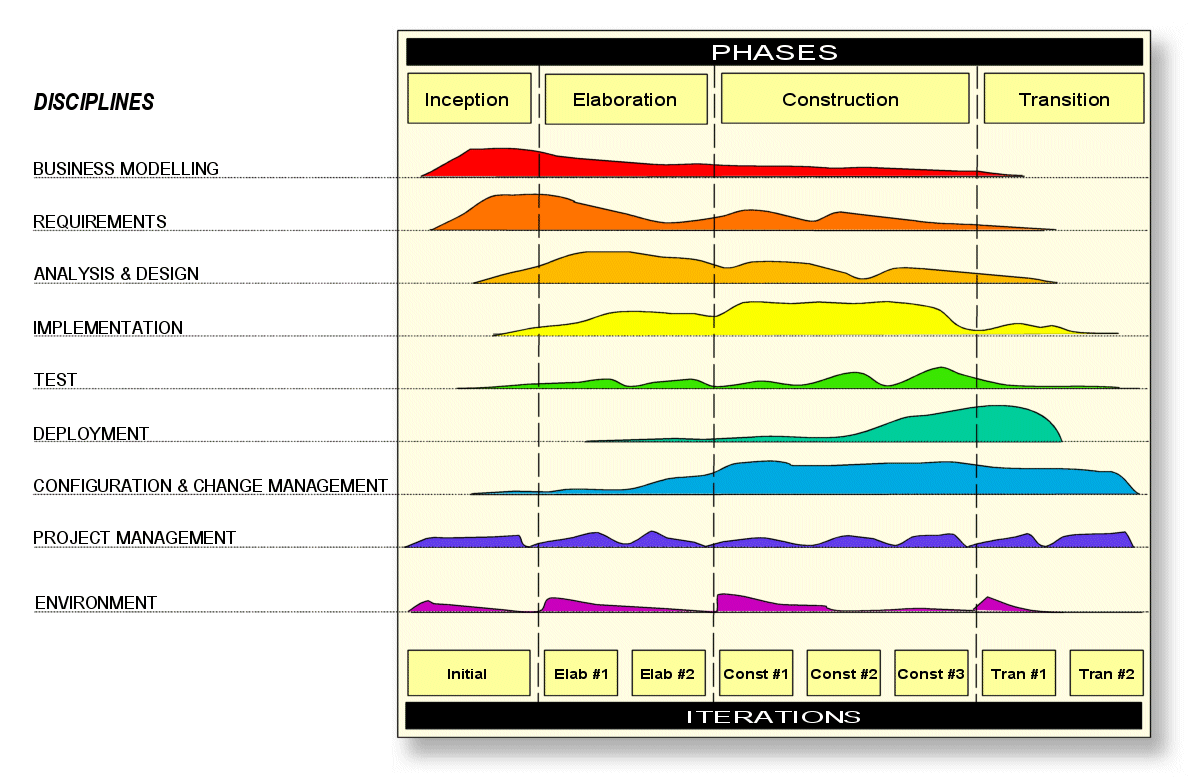
\includegraphics[width=0.80\textwidth]{Billeder/Udviklingsproces/RUP}
	\caption{RUP model}
	\label{fig:rup}
\end{figure}

\textbf{Inception}\\
Inception fasen er projektets indledende fase, og bruges til at lave forundersøgelse, valg af hardware/software samt opsætning af krav. I løbet af inception fasen udarbejdes foranalyse, indkøbsliste, krav til systemet og overordnet systemskitse. 

\textbf{Elaboration}\\
Elaboration fasen tager hånd om systemarkitektur og design. I denne fase udarbejdes der indledningsvis en domain model og derefter systemarkitektur af hardware og software. 

\textbf{Construction}\\
I construction fasen er produktet i fokus, og der skiftes løbende mellem implementering af ny funktionalitet, test og dokumentation af nytilføjet funktionalitet. 

\textbf{Transition}\\
Transition er den afsluttende fase, og tager hånd om færdiggørelse af projekt og overdragelse af produkt. Idet gruppen ikke har nogen egentlig kunde, bruges fasen til lave accepttest, færdiggøre dokumentation og udarbejdelse af rapport. 

\newpage

\subsubsection*{ASE modellen}
ASE modellen som ses på figur \ref{fig:dokument_udvikling} er brugt i kombination med RUP. RUP bruges til at danne overordnede rammer for projektet, mens ASE modellen bruges til definere hvilke dokumenter der skal udarbejdes og hvornår. På figur \ref{fig:dokument_udvikling} vise hvilke dokumenter der oprettes som produkt af ASE modellen. 

\begin{figure}[H]
	\centering
	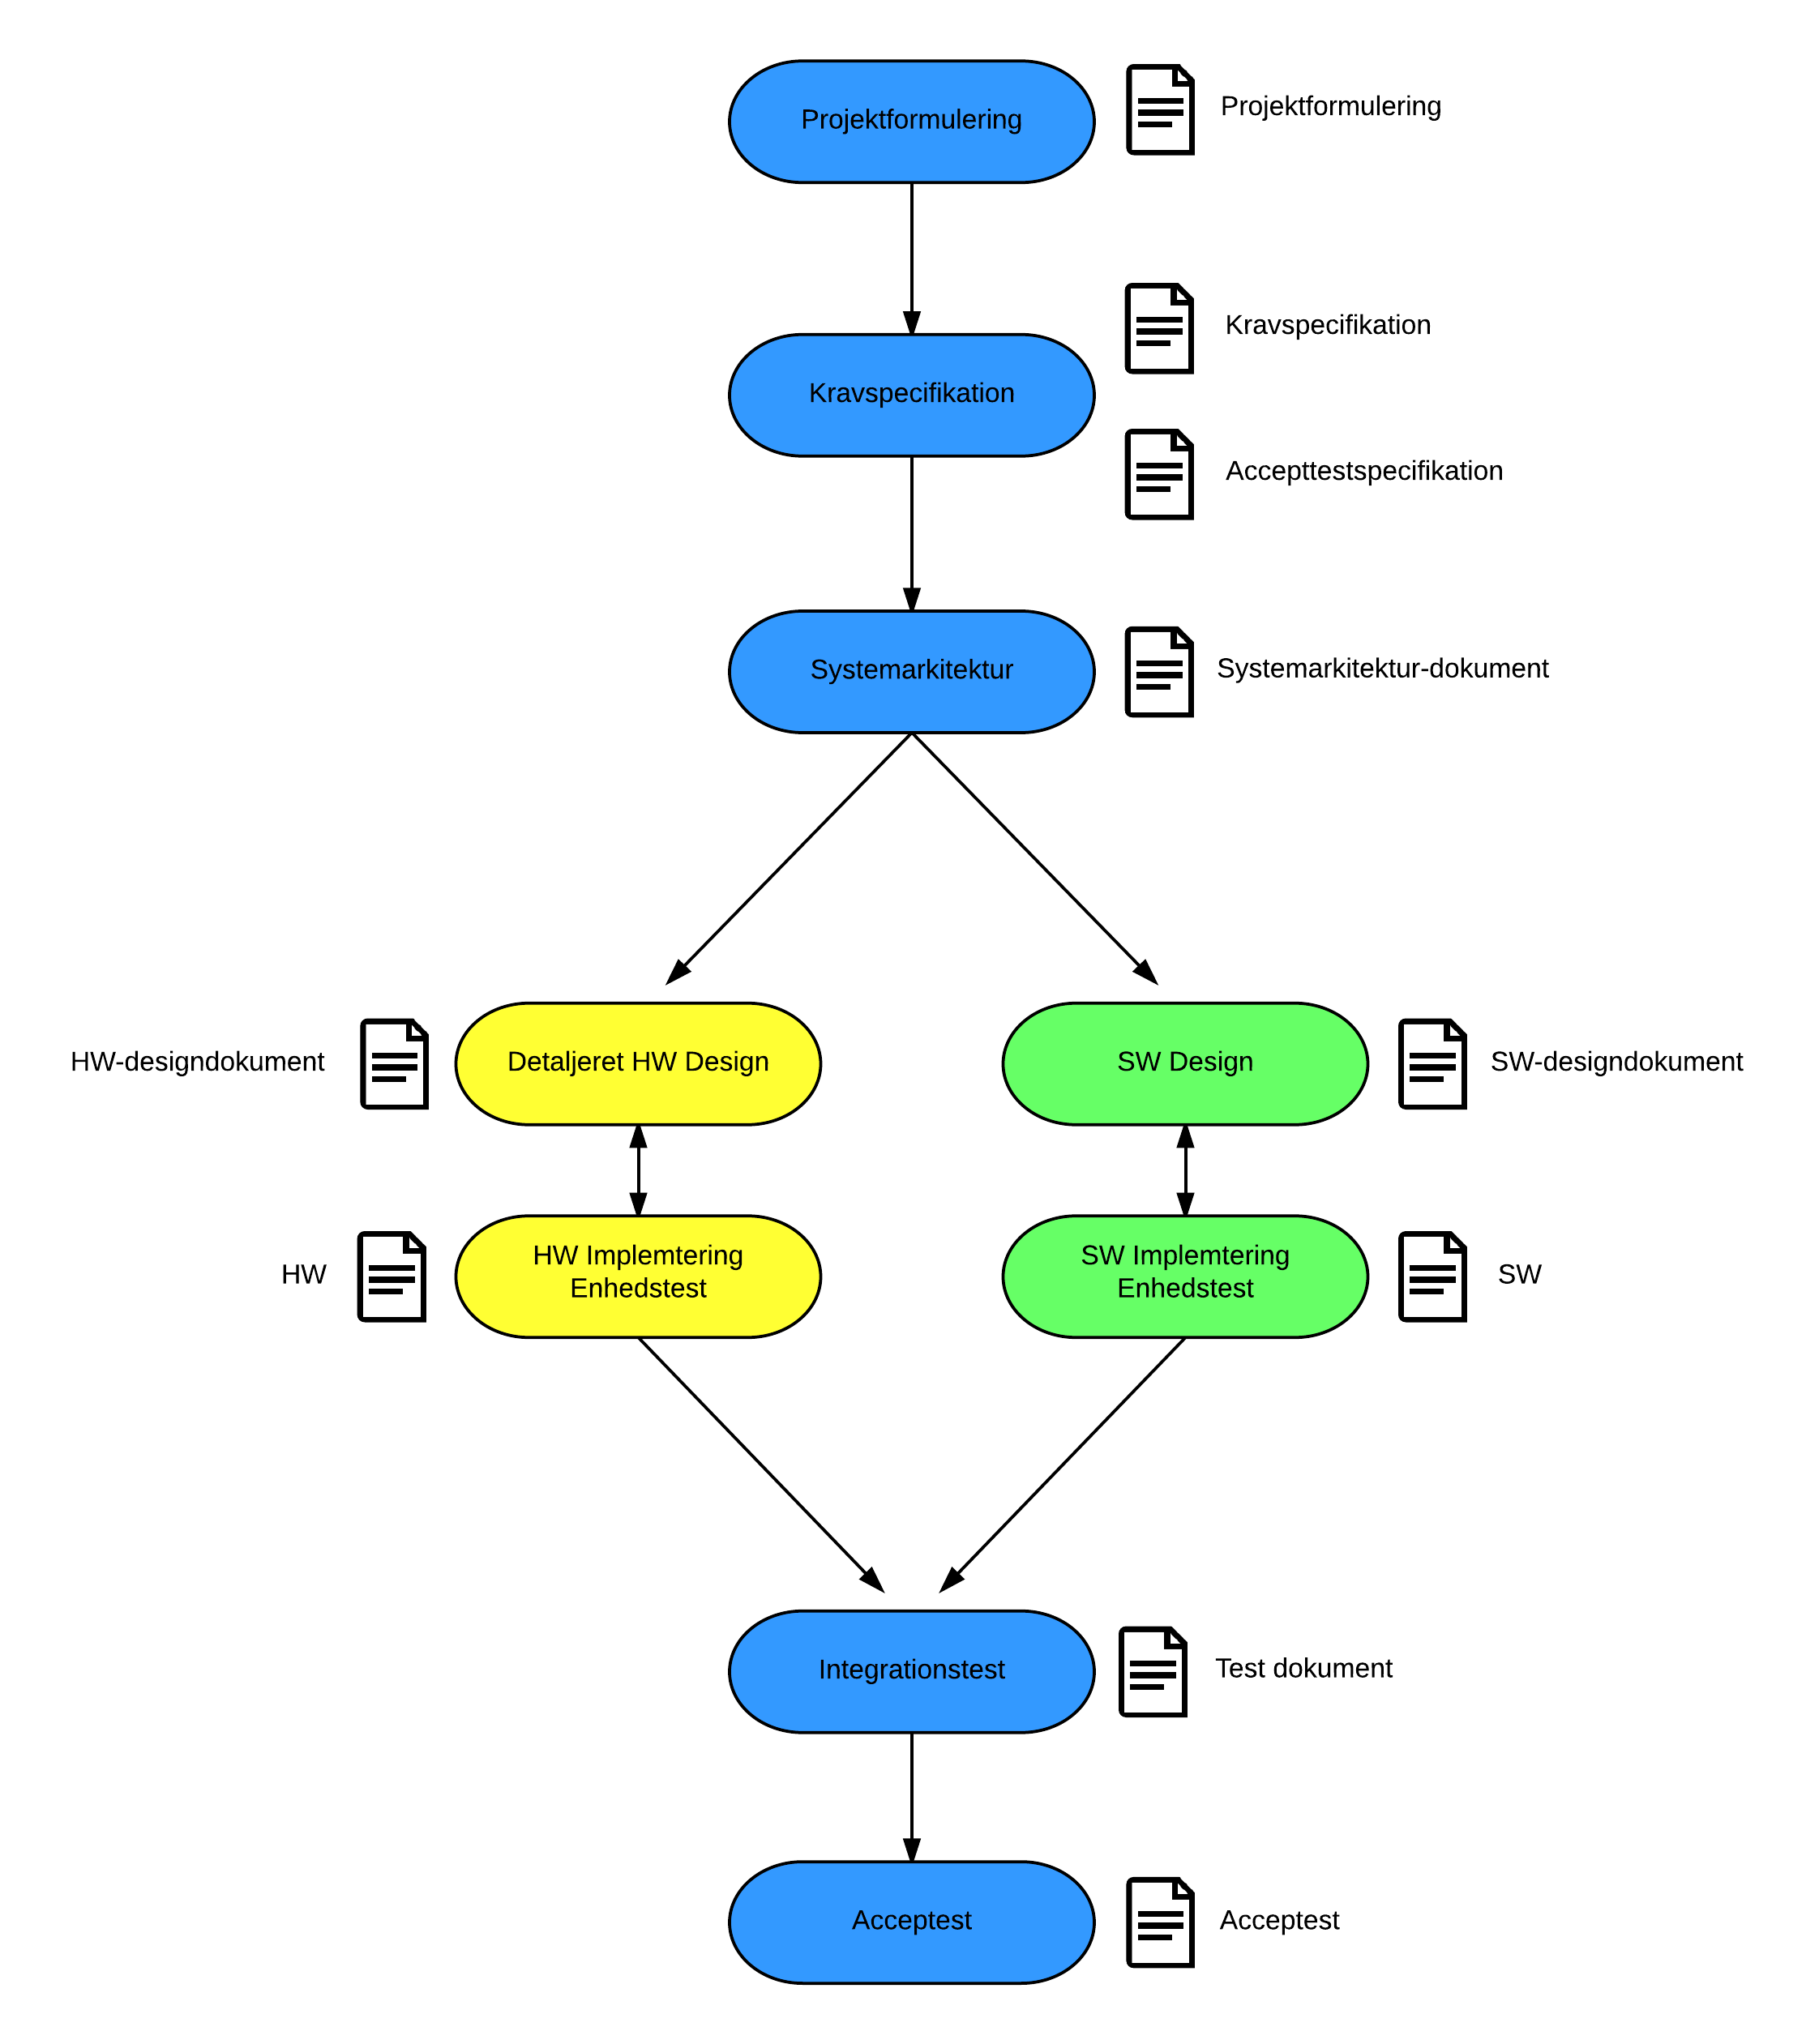
\includegraphics[width=1\textwidth]{Billeder/Udviklingsproces/ase_model}
	\caption{ASE modellen}
	\label{fig:dokument_udvikling}
\end{figure}

\newpage

\subsubsection*{N + 1 model}
Alt software design i projektet er lavet ud fra systemudviklings modellen N + 1 [X]. Modellen er en udviklingsmodel der beskriver software fra flere forskellige view's.  
Med N + 1 modellen tages der udgangspunkt i et use case view. Derefter er det op til udviklerholdet at bestemme hvor mange views der skal bruges for at beskrive systemet på tilstrækkelig vis. 

Til beskrivelse af systemets software anvendes en 5 + 1 view model, som indeholder use case view, logical view, process view, data view, deployment view og implementation view. 
På figur \ref{fig:n+1} ses en illustration der viser 5 + 1 modellen.
5 + 1 modellens view's beskrives uddybende på den følgende side. 

\begin{figure}[H]
	\centering
	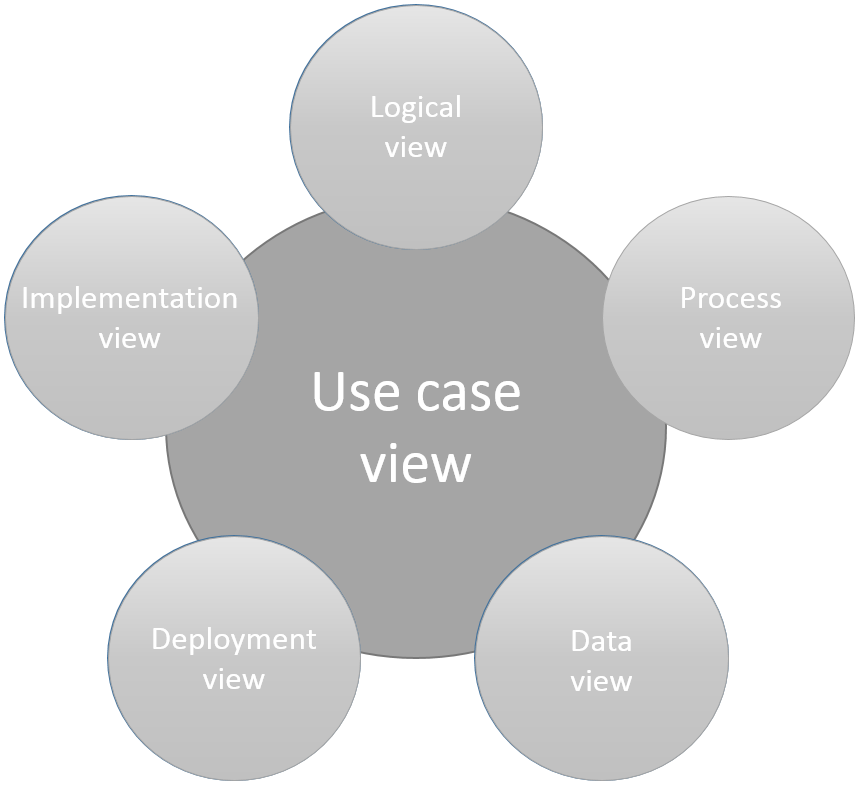
\includegraphics[width=0.7\textwidth]{Billeder/Udviklingsproces/n+1}
	\caption{5 + 1 model}
	\label{fig:n+1}
\end{figure}

\newpage


\textbf{Use case view}\\
Use case viewet består af use case beskrivelser, der er udviklet ud fra brugers synspunkt og som bruges til at beskrive systemets funktionalitet og forskellige brugsscenarier. Alle udarbejdede use case beskrivelser forefindes i kravspecifikationen.

\textbf{Logical View}\\
Logical view bruges til at beskrive de logiske blokke i systemet. På baggrund af hver iteration, er der udarbejdet tilhørende designoverview-, pakke-, klasse-, sekvens- og state machine diagrammer. Diagrammerne bruges til at give et overblik over systemets funktionalitet på et mere detaljeret niveau.

\textbf{Process View}\\
Process view bruges til at beskrive sideløbende processer/tråde i systemet og hvordan samspillet imellem disse er. I view'et beskrives også krav til timing i kommunikation mellem drone og server.

\textbf{Data View}\\
I data viewet beskrives layout af data der gemmes i systemet og hvordan det lagres. Desuden beskrives hvordan data sendes rundt i systemet og hvordan servers database tilgås.

\textbf{Deployment View}\\
Deployment view beskriver systemets grundlæggende fysiske elementer og sammenspillet mellem dem. I view'et beskrives også hvilke software pakker der bruges i systemet og hvor de bruges. Desuden beskrives hvilke protokoller der er anvendt, fx. layout af meddelelser med header/start/stop

\textbf{Implementation View}\\
Implementation view beskriver vigtige elementer i systemet som ikke er blevet beskrevet i andre views. Bla. beskrives hvilke værktøjer der er benyttet til projektet og hvordan disse værktøjer er sat op. Det beskrives også hvilke filer systemet er bygget af og hvordan disse filer skal linkes sammen.


\newpage
\subsection{Udviklingsværktøjer}
I dette afsnit beskrives de udviklingsværktøjer [X] der er benyttet i løbet af projektet. \\

\textbf{Latex}\\
Latex er benyttet til udarbejdelse af dokumentation og rapport. 

\textbf{Git}\\
Git er versionsstyring og fildelings værktøj.

\textbf{Lucidchart}\\
Lucidchart er benyttet til udarbejdelse af software diagrammer.

\textbf{Visio}\\
Visio er benyttet til udarbejdelse af hardware diagrammer.

\textbf{Atmel studio 6.2}\\
Atmel studio er det IDE hvor kode til main controller skrives.

\textbf{Arduino IDE}\\
Arduino IDE er brugt til at teste kode til main controller.

\textbf{Atom}\\
Atom er et IDE / tekstbehandlings program til håndtering kode.

\textbf{OSX ternimal}\\
Opsætning og programmering af server og webapplikation. 

\textbf{SQLite database}\\
SQLite er benyttet til systemets database.

\newpage
\section{Systemarkitektur}
\label{chap:systemarkitektur}

Domain modellen anvendes som en overgang mellem kravspecifikation og systemarkitektur.
I kravspecifikation beskrives hvad der sker ved interaktion med systemet. Mens
systemarkitekturen bruges til at beskrive systemet i blokke og til at skitsere både interne
og eksterne forbindelser. Domain modellen bruges til at beskrive hele systemets domæne.
Der kigges ikke på hardware vs. software, der kigges i stedet på "enheder"og deres
ansvarsområder.\\

\begin{figure}[H]
	\centering
	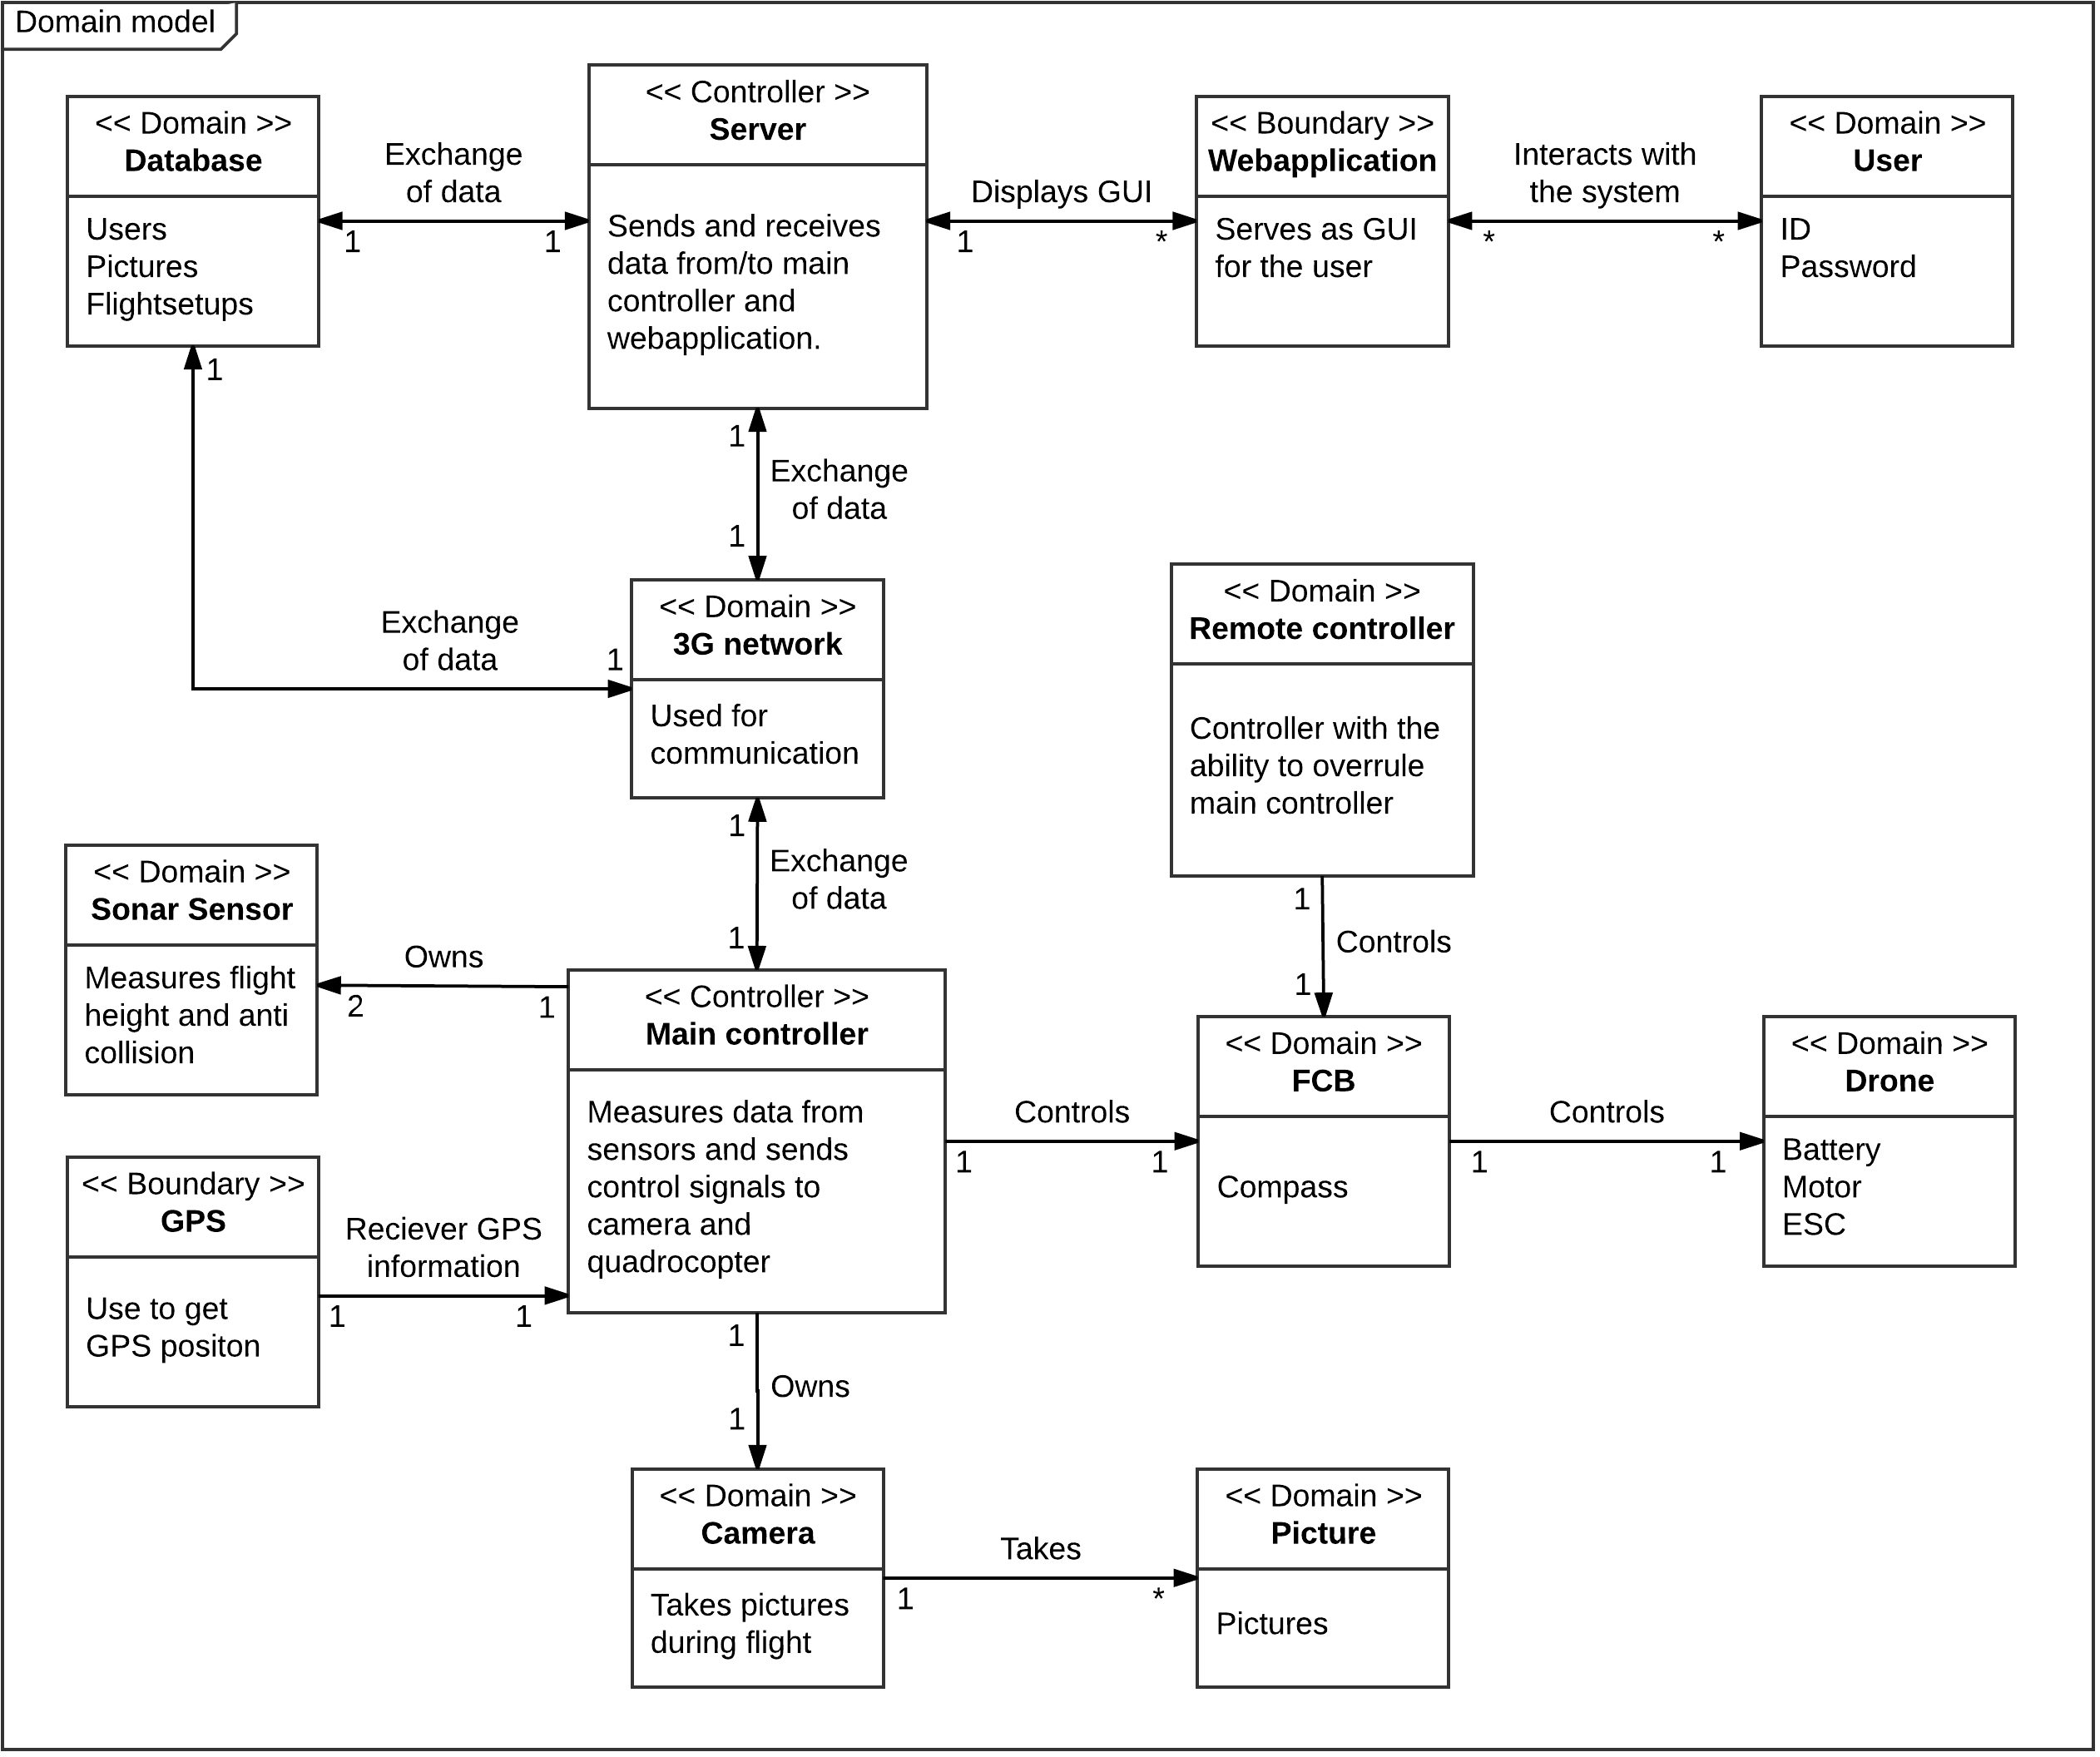
\includegraphics[width=1\textwidth]{Billeder/domain_model.png}
	\caption{Domain model}
	\label{fig:domain}
\end{figure}


\newpage

Efter at have udarbejdet kravspecifikation, systemskitse og domain model, var der formet en ide om hvordan systemet skulle fungere. I det følgende beskrives hvordan systemarkitekturen er udformet. 


Systemarkitekturen er udført ved brug af SysML og UML diagrammer. 
SysML bruges til beskrivelse af systemets hardware i blokke og som samlet system. Ud fra N + 1 og applikations modellen udformes UML diagrammer, der bruges til beskrivelse af systemets software. 
Foruden SysML og UML diagrammer benyttes en række andre diagrammer, i det følgende beskrives nogle af de mest centrale diagrammer.\\


\textbf{Use case}\\
Use cases og tilhørende diagrammer er benyttet i projektforløbets indledende faser. De bruges til at definere systemets kunnen og opdele systemet i mindre dele. Use cases har i høj grad fungeret som et omdrejningspunkt, hvorfra alt funktionalitet udspringer. \\


\textbf{SysML}\\
Der er benyttet to slags SysML diagrammer til dokumentation af systemets hardware. Block definition diagrammer (bdd'er) er brugt til at identificere og beskrive systemets hardware blokke og deres indbyrdes forhold. Internal block diagrammer (ibd'er) er brugt til at vise de identificerede blokkes interne og eksterne forbindelse, hvordan blokkene kommunikerer og hvilke signaler der flyder imellem dem. \\


\textbf{UML}\\
Der er benyttet fire slags UML diagrammer til dokumentation af systemets software.
På baggrund af use cases og domain modellen udformes pakkediagrammer, der bruges til at beskrive ansvarsområder i systemet. Sekvensdiagrammer bruges til at identificere systemets klasser, klassernes metoder samt timing i systemet. Klasser samt tilhørende metoder og attributter beskrives ved hjælp af klassediagrammer. State machines bruges til at beskrive flow mellem forskellige states. 


\newpage

\subsection{Hardware}
I dette afsnit beskrives hvordan systemets hardwarearkitektur er udformet vha. SysML diagrammer. Indledningsvis bruges block definition diagrammer til at identificere og beskrive systemets blokke. Senere åbnes udvalgte blokke og de interne og eksterne forbindelser vises med internal block diagrammer. 


\subsubsection*{Block definition diagram}

Det overordnede bdd på figur \ref{fig:bdd_asd} viser hvilke hardware blokke systemet består af, samt hvilke parts blokkene indeholder.

\begin{figure}[H]
	\centering
	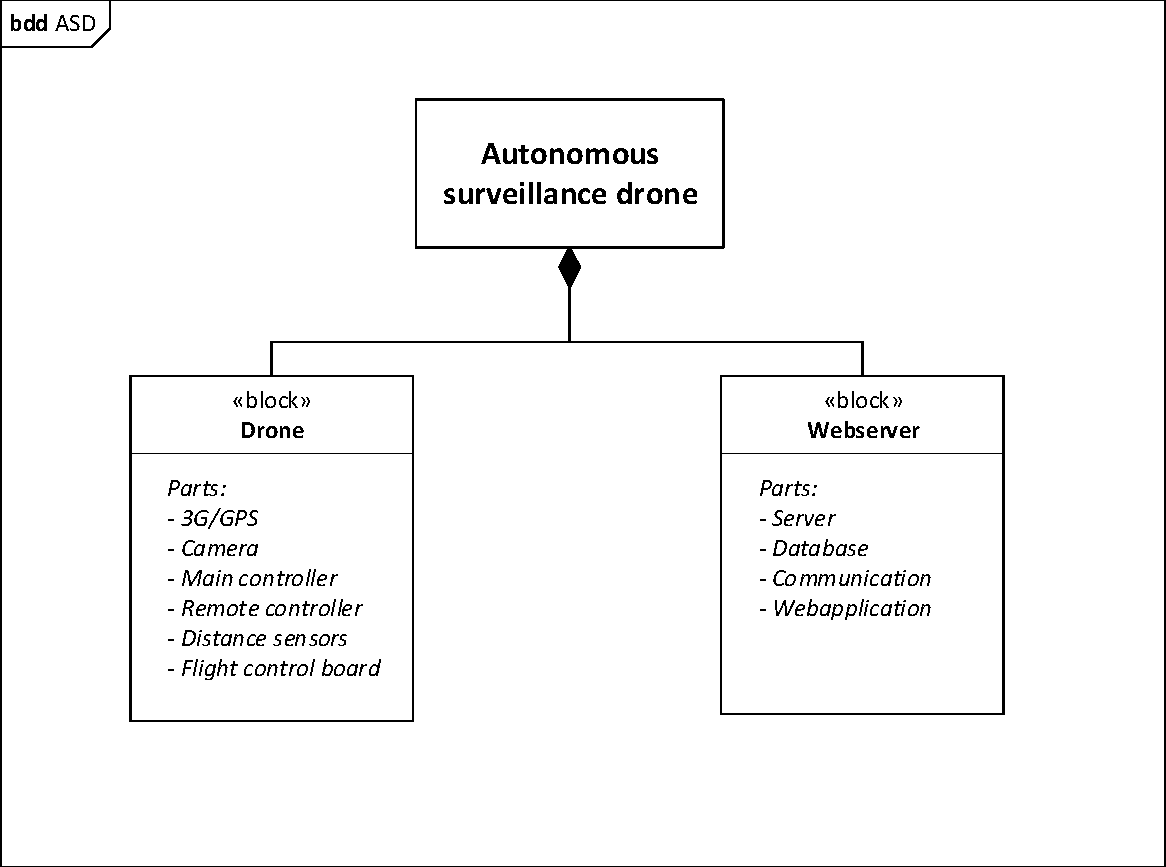
\includegraphics[width=1.0\textwidth]{Billeder/Projektbeskrivelse/bdd_overordnet.pdf}
	\caption{Overordnet bdd for systemet}
	\label{fig:bdd_asd}
\end{figure}

\textbf{Drone} \\
Drone blokken indeholder alle de hardwareenheder der giver funktionalitet til drone. Beskrivelse af de eksterne og interne forbindelser mellem de forskellige parts er beskrevet nærmere med ibd'er. \\

\textbf{Webserver} \\
Webserver blokken indeholder server, database, communication og webapplikationen.

\newpage

\subsubsection*{Internal block diagram}
\vspace{-0.3cm}	

På figur \ref{fig:ibd_asd} vises et overordnet ibd for systemet. Det overornede ibd viser hvordan systemets største blokke kommunikerer med hinanden og hvilken type signaler der anvendes mellem blokkene. 

\begin{figure}[H]
	\centering
	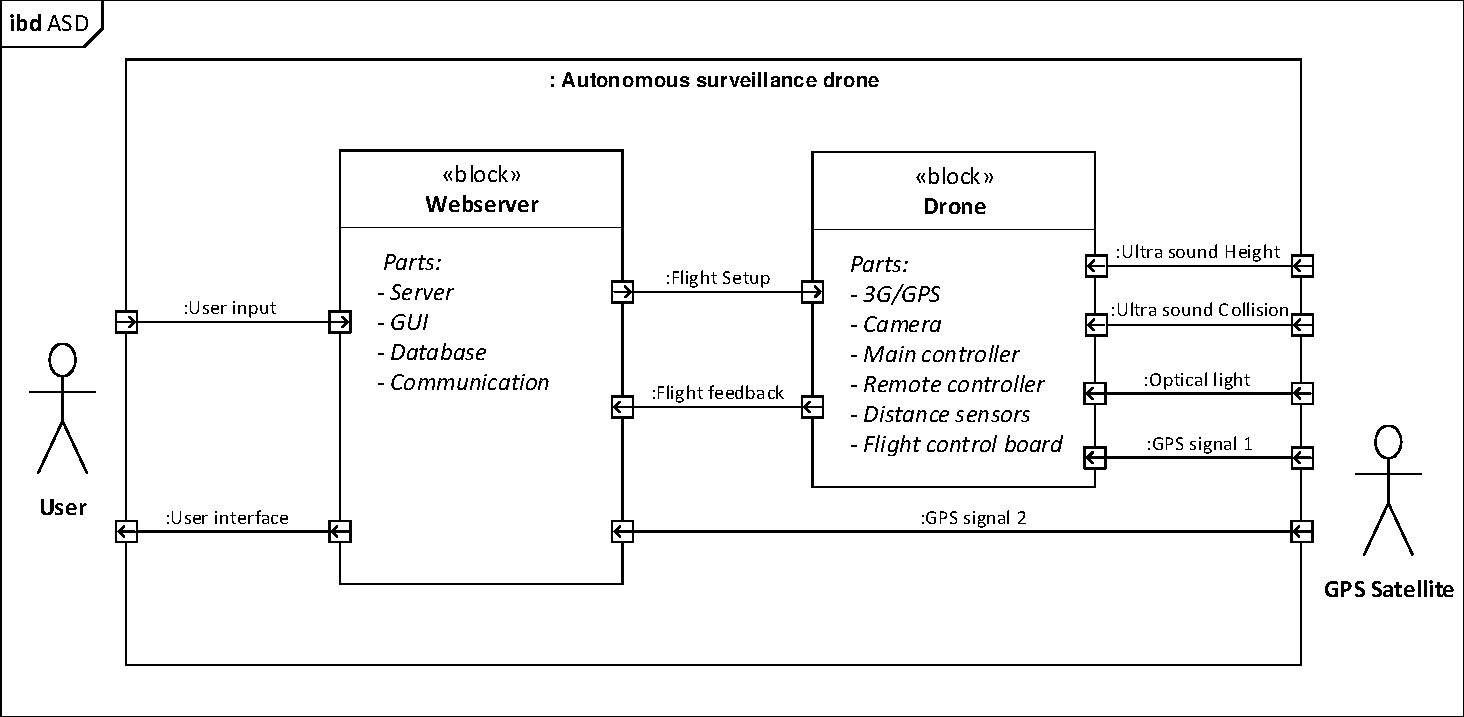
\includegraphics[width=1\textwidth]{Billeder/Projektbeskrivelse/ibd1_overordnet.pdf}
	\caption{Overordnet ibd for systemet}
	\label{fig:ibd_asd}
\end{figure}

Da drone blokken er stor og indeholder mange part kræves yderlige beskrivelse. På den følgende side åbnes drone blokken og de interne forbindelser i blokken vises.

\newpage


På figur \ref{fig:ibd_drone} vises et ibd, der går mere i dybden med drone blokken. ibd'et åbner drone blokken og viser hvordan parts i drone blokken kommunikerer med hinanden. 

\begin{figure}[H]
	\centering
	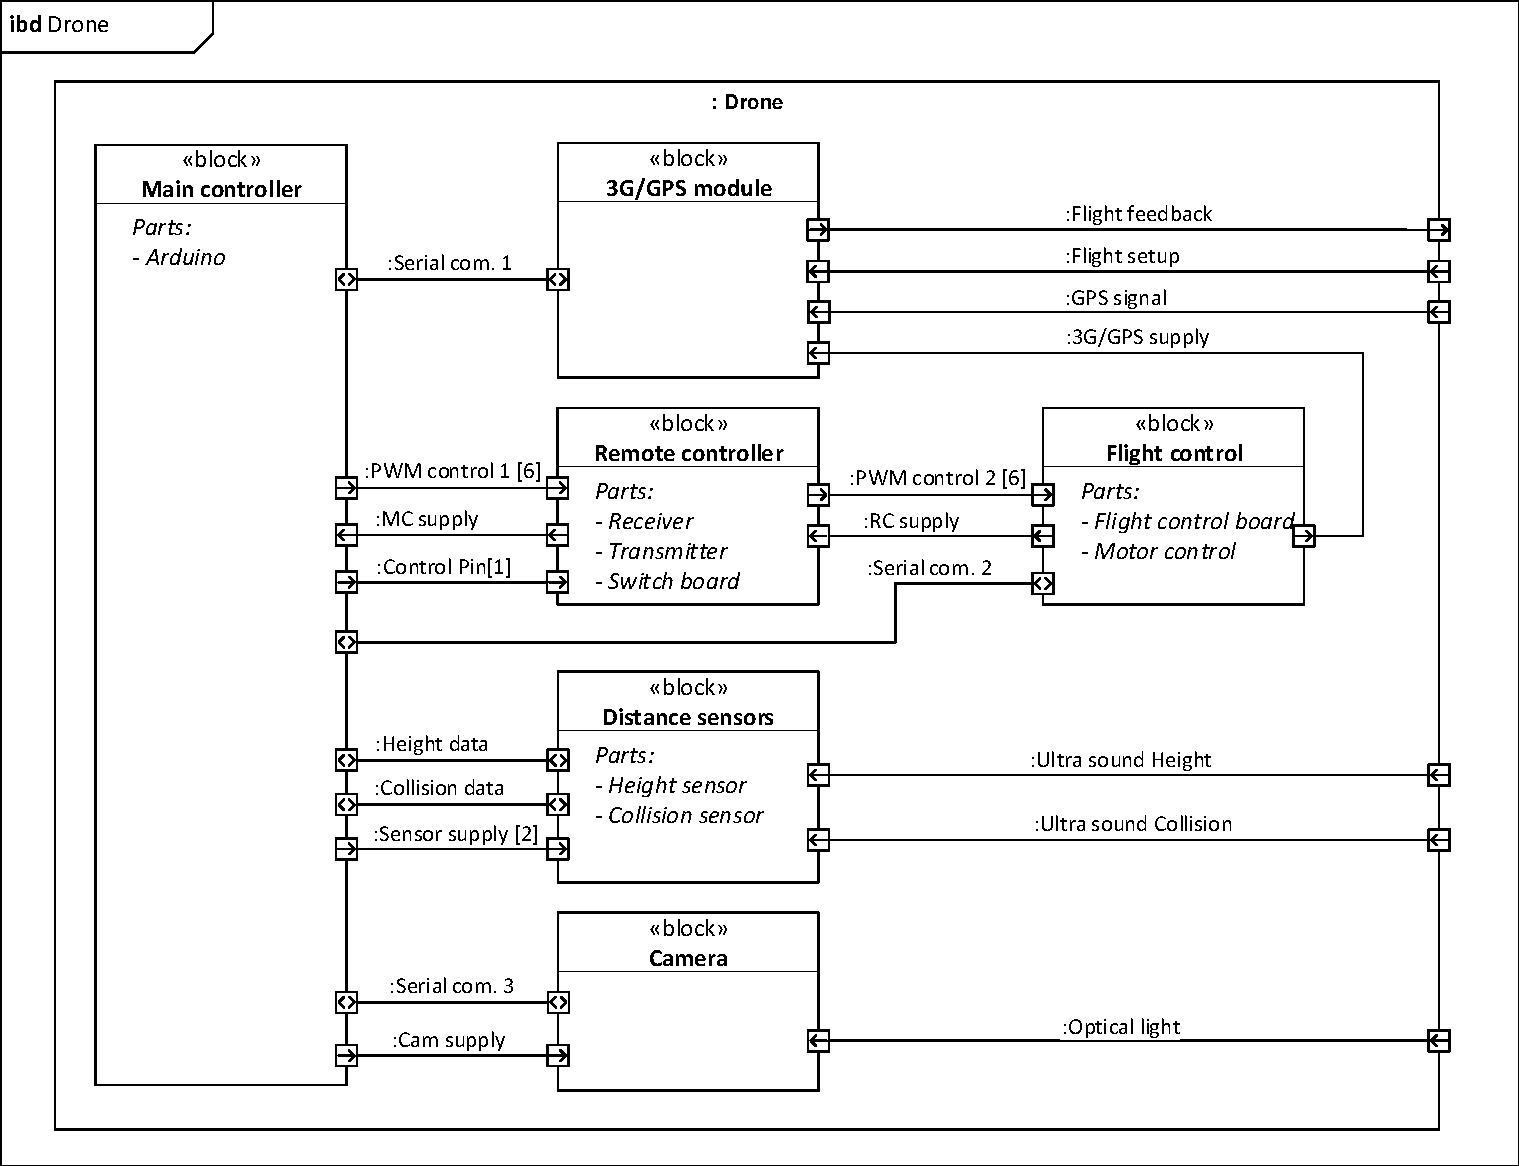
\includegraphics[width=1\textwidth]{Billeder/Projektbeskrivelse/ibd2_drone.pdf}
	\caption{ibd drone}
	\label{fig:ibd_drone}
\end{figure}


For yderlige beskrivelser af parts fra drone blokken henvises til ibd'er i hardwarearkitektur [3].
Der vises ikke udvidede ibd'er for webserver, da webserver ikke indeholder hardware og derfor beskrives nærmere ved brug af UML diagrammer i software afsnittet.



\newpage

\subsection{Software}

I dette afsnit beskrives hvordan softwarearkitekturen ved brug af N+1 og applikations modellen tager udgangspunkt i use cases og ender ud i detaljerede klassedigrammer. 
   
\subsubsection*{Pakkediagrammer}
\vspace{-0.3cm}	
Indledningsvis identificeres pakkediagrammer ud fra use cases og domain modellen. På figur \ref{fig:package_drone} vises et pakkediagram tilhørende dronens software. Pakkerne i pakkediagrammet bruges til at definere de forskellige ansvarsområder i systemts software. For nærmere beskrivelser af pakkediagrammer over systemets software henvises til logical view [4].
 
\begin{figure}[H]
	\centering
	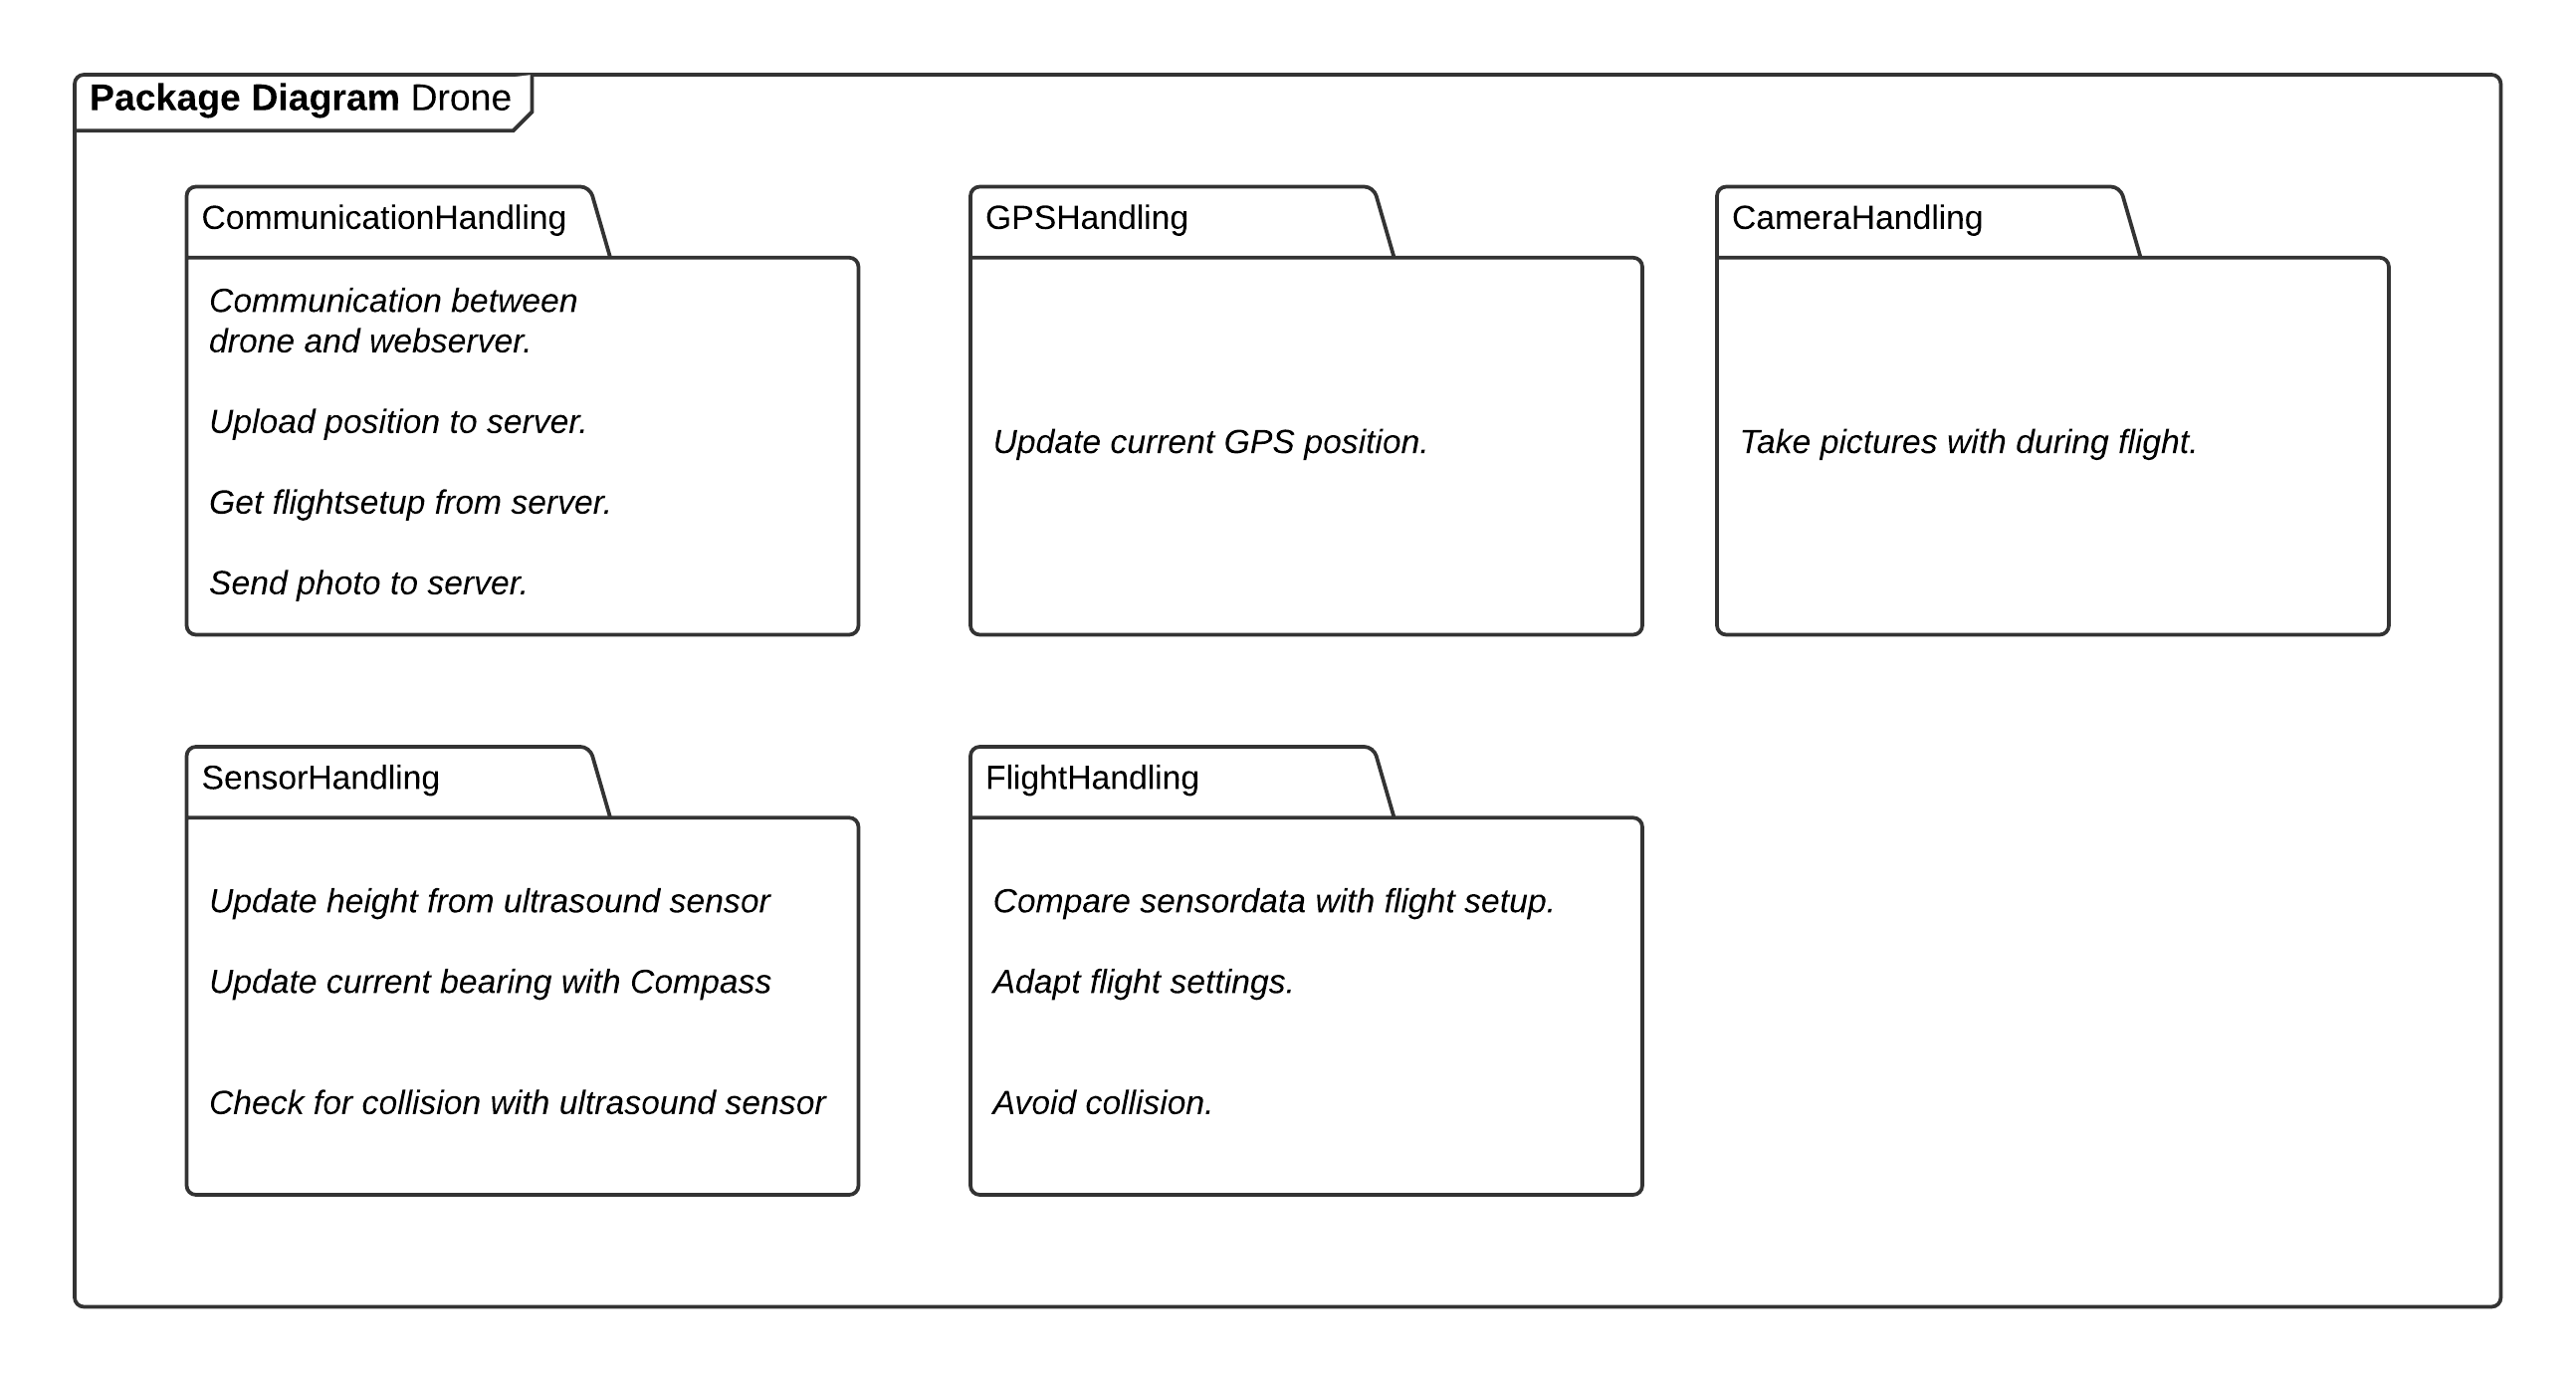
\includegraphics[width=1\textwidth]{Billeder/Projektbeskrivelse/Packagediagram_drone}
	\vspace{-0.9cm}	
	\caption{Overordnet pakkediagram for drone}
	\label{fig:package_drone}
\end{figure}

\newpage

\subsubsection*{Sekvensdiagrammer}
\vspace{-0.3cm}	

Efter at have udformet pakkediagrammer påbegyndes udformning af sekvensdiagrammer. Disse diagrammer bruges til at identificere softwareklasser, klassernes metoder, klassernes indbyrdes forhold, samt timing i systemet. Enheder der indgår i sekvensdiagrammerne tages ud fra domain modellen. 

Sekvensdiagrammet på figur \ref{fig:login_flysetting} viser et eksempel på en use case omsat til et sekvensdiagram. Sekvensdiagrammet bruges til overordnet at vise hvordan bruger interagerer med webapplikation når der laves ny flyveopsætning. For yderlige beskrivelser af sekvensdiagrammer tilhørende systemet henvises til logical view [4].

 
\begin{figure}[H]
	\centering
	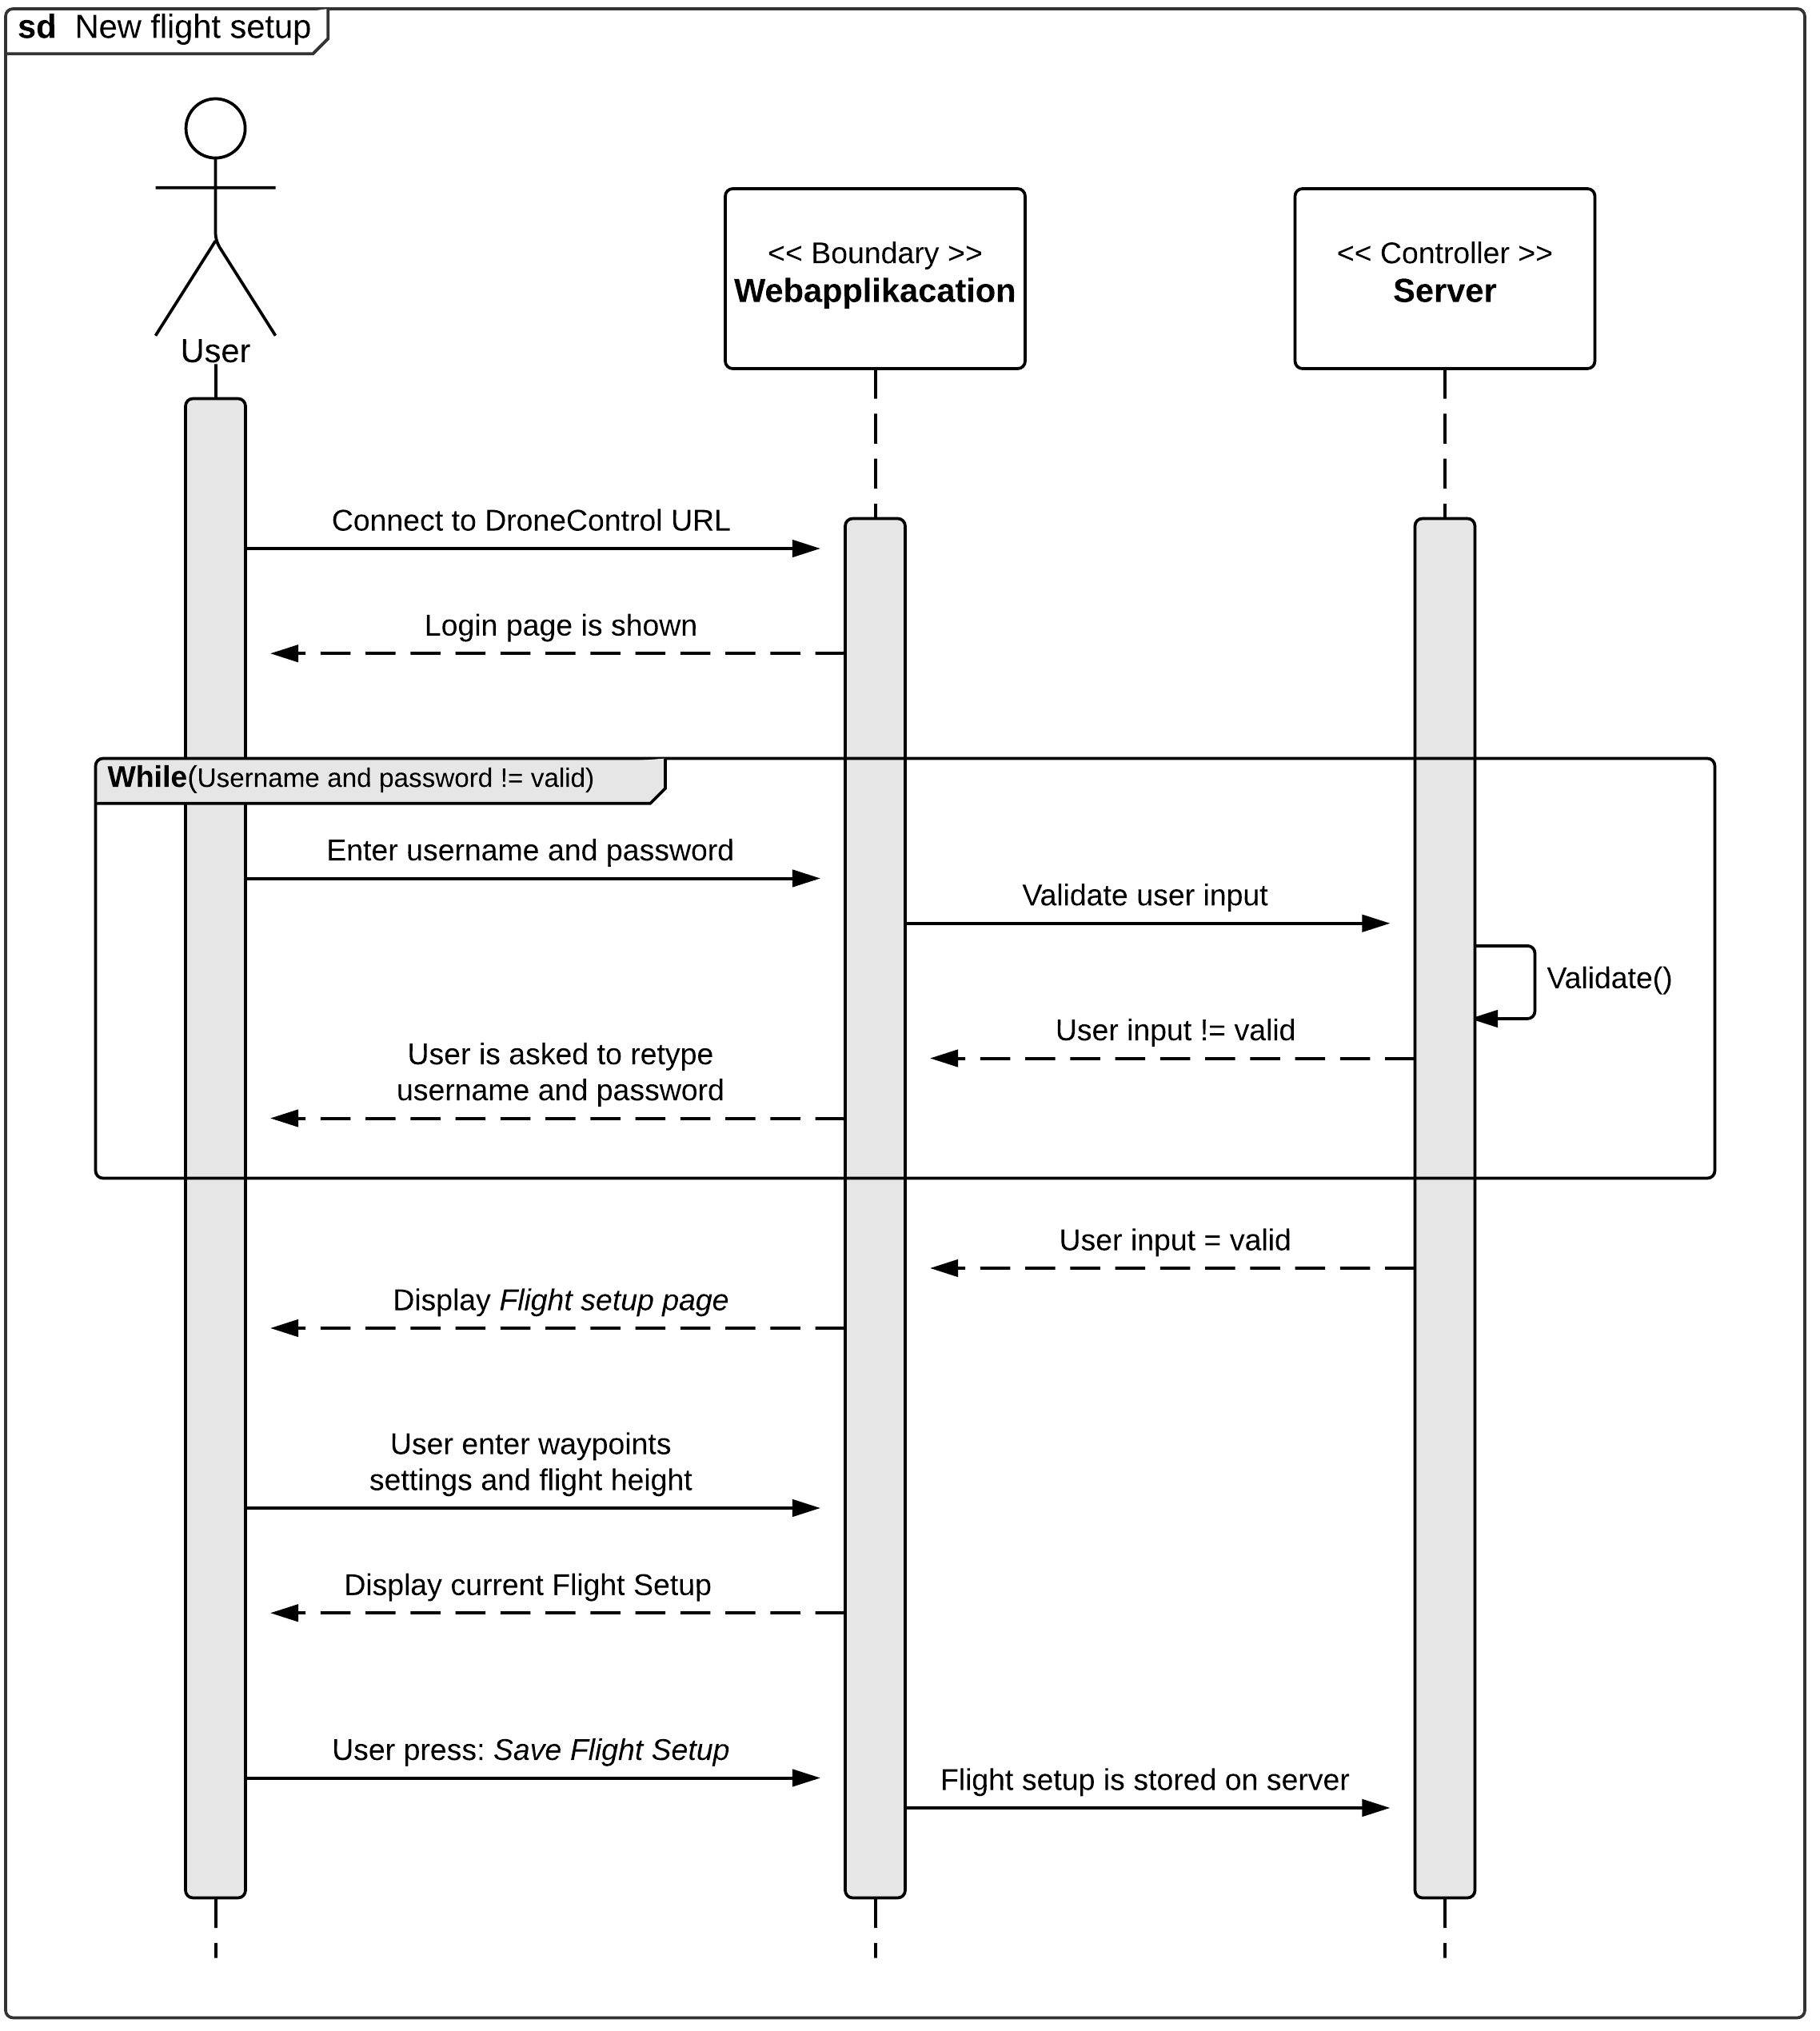
\includegraphics[width=1\textwidth]{Billeder/sekvens.png}
	\vspace{-0.6cm}	
	\caption{Sekvensdiagram - ny flyveopsætning}
	\label{fig:login_flysetting}
\end{figure}

\newpage
\subsubsection*{Klassediagrammer}
\vspace{-0.3cm}	

Efter at have udformet sekvensdiagrammer er der opbygget et vist kendskab til de forskellige klasser, deres metoder og deres indbyrdes forhold. For på overskuelig vis at illustrere og beskrive systemets softwareklasser laves klassediagrammer.

På figur \ref{fig:class_drone} vises et klassediagram tilhørende dronens software. Bemærk at klassediagrammet er fra første iteration, hvilket betyder det er relativt lille og ikke indeholder så mange klasser og metoder. For mere information om de enkelte klasser og deres ansvarsområder henvises til logical view [4].

\begin{figure}[H]
	\centering
	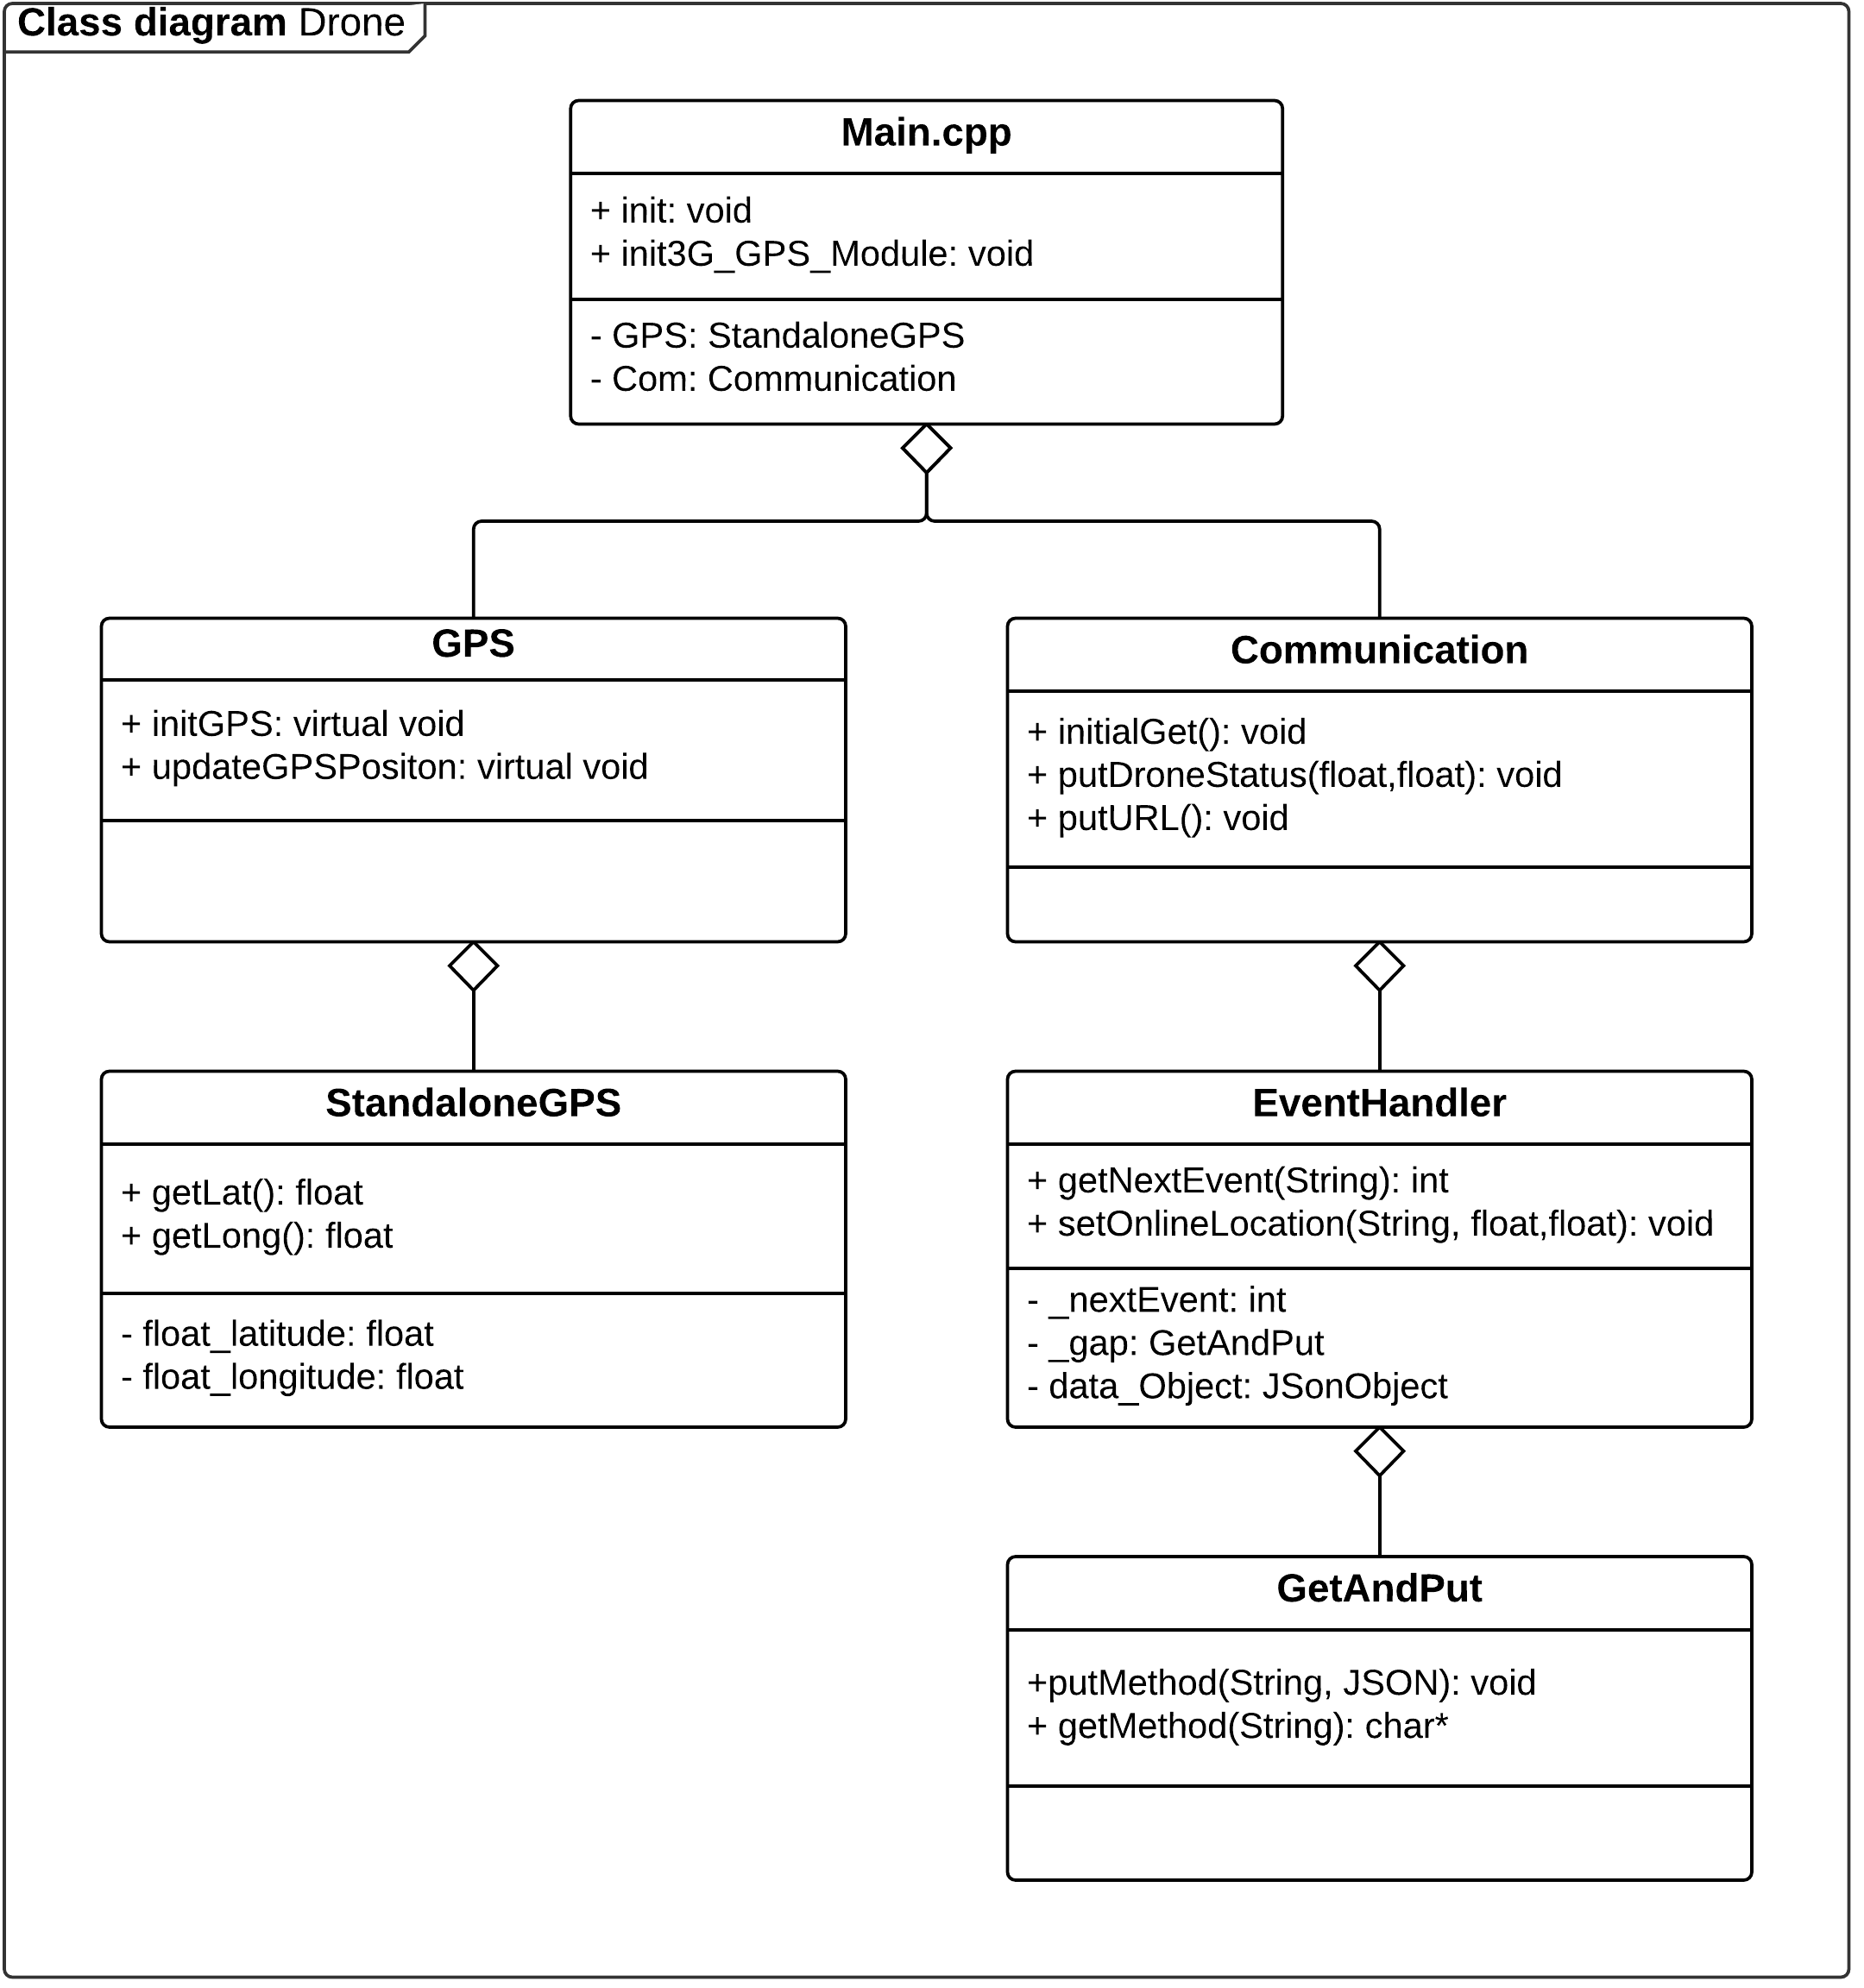
\includegraphics[width=1\textwidth]{Billeder/classdiagram.png}
	\vspace{-0.6cm}	
	\caption{Klassediagram drone}
	\label{fig:class_drone}

\end{figure}


\newpage
%%%%%% Design %%%%%%
\section{Design}

I dette afsnit beskrives systemets design. Systemet indeholder overordnet set de tre enheder drone, server og webapplikation samt en kommunikations protokol derimellem. Drone bruges til at overvåge og tage billeder, server står for håndtering af data, og webapplikation er systemets grænseflade til bruger. Mellem drone/server og webapplikation/server gøres brug af HTTP protokollen til kommunikation og udveksling af data.



\subsection{Drone}

Systemets bruger er ansvarlig for at lave flyveopsætninger, som indeholder informationer om det område drone skal overvåge.

Når drone tændes skal den løbende og uden menneskelig indblanding kontrollere om der er en ny flyveopsætning tilgængelig på server. Hvis der er en ny flyveopsætning tilgængelig hentes den, og en ny flyvning påbegyndes. 

Under flyvning flyver drone på egen hånd til de definerede GPS positioner. Afhængig af om bruger har valgt om der skal tages billeder eller ej, tager dronen billeder som via mobilt netværk sendes til server. 
Under flyvning kontrollerer drone løbende egen GPS position, flyvehøjde og flyveretning. Dette gør dronen for løbende at kunne tilpasse flyvehøjde og orientering og for at kunne sende information om nuværende GPS position til server.

På figur \ref{fig:class_drone} vises et simplificeret klasse diagram for drone. I det viste klassediagram vises softwareklasser og deres indbyrdes forhold. For yderlige information om de enkelte klasser, deres metoder og deres ansvarsområder henvises til logical view i \textit{Systemarkitektur og Design} i dokumentationen. [xx]

\begin{figure}[H]
\centering
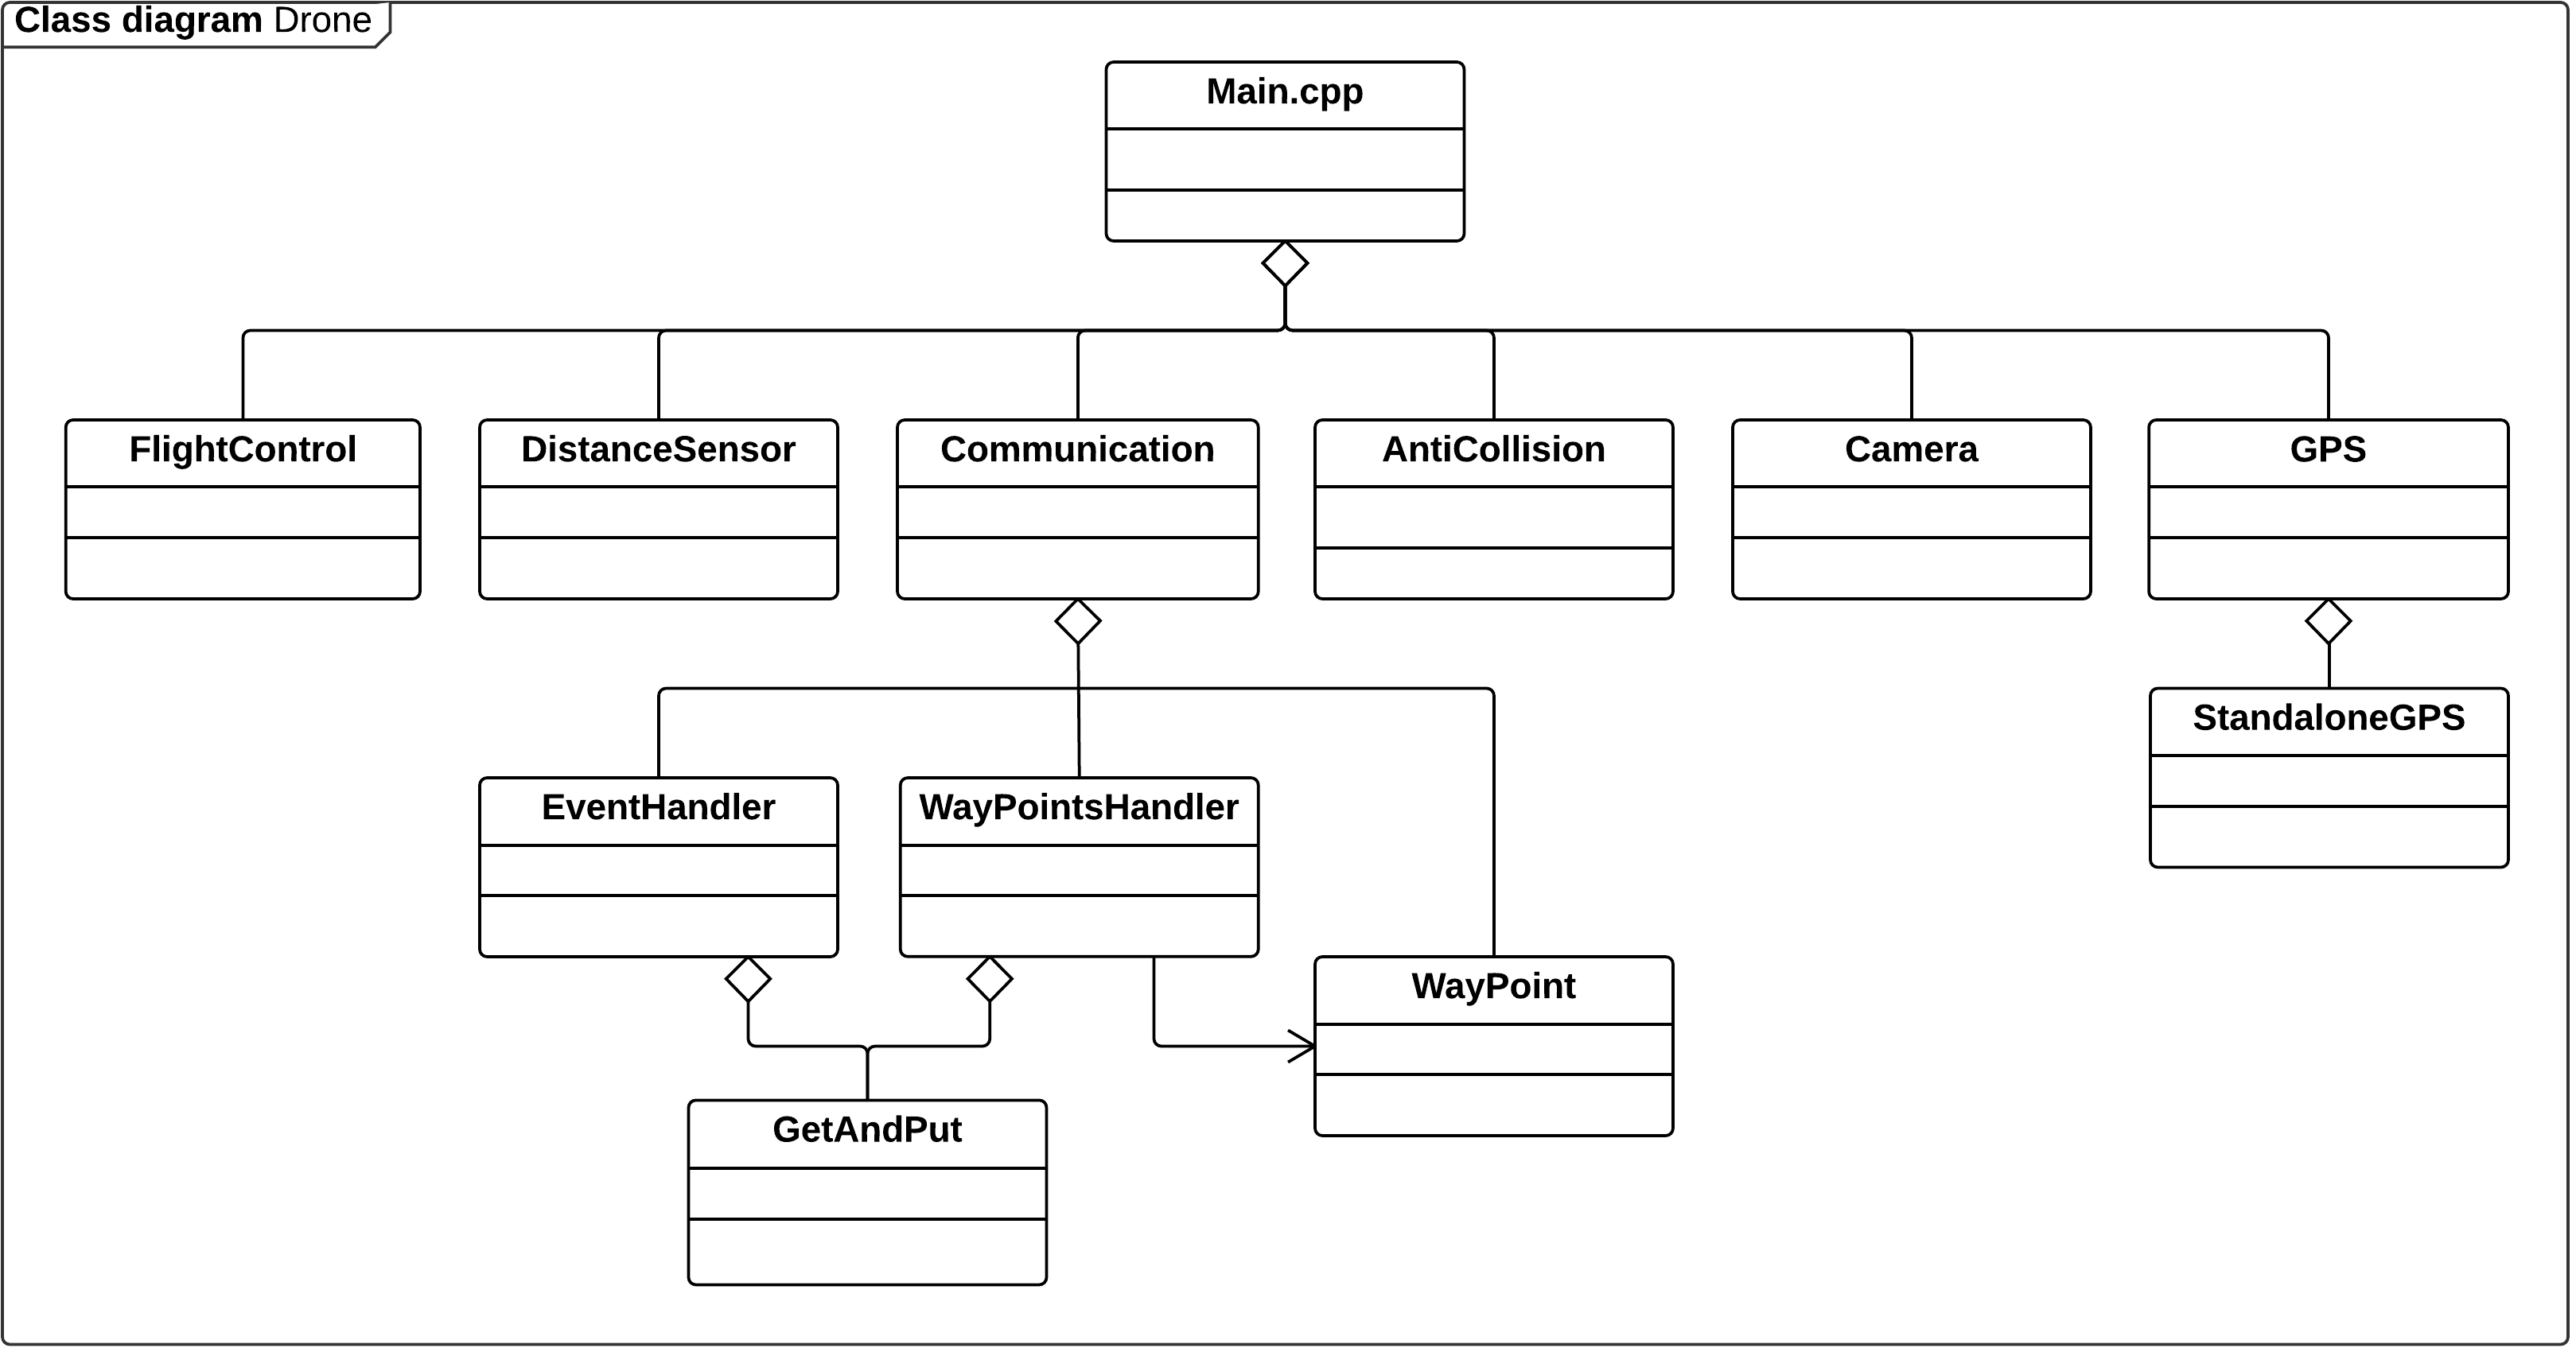
\includegraphics[width=1\textwidth]{Billeder/Design_Class_drone.png}
\vspace{-0.5cm}
\caption{Klassediagram drone}
\label{fig:class_drone}
\end{figure}


\newpage 

\subsection{Server}

Server består af SQLite database med et tilhørende REST API. I SQLite databasen gemmes og hentes løbende information om systemets brugere, samt information om flyveopsætninger, flyveruter og billeder.  

Server er en passiv enhed, som er ansvarlig for håndtering af systemets data. Server tager aldrig initiativ til udveksling af data, den står i stedet og venter på at blive igangsat af enten drone eller webapplikation.

For systemets bruger kan det se ud som om udveksling af data og information går direkte fra webapplikation til drone eller omvendt. Men reelt set er webapplikation og drone aldrig i direkte kontakt med hinanden. I stedet går al kommunikation til og fra server via HTTP protokollen. 

På figur \ref{fig:deployment_diagram} ses et deployment diagram, der viser hvordan drone og webapplikation kommunikerer med server for at hente og gemme information. For yderlige information om server og tilhørende SQLite database henvises til data view i \textit{Systemarkitektur og Design} i dokumentationen [xx].

\begin{figure}[H]
\centering
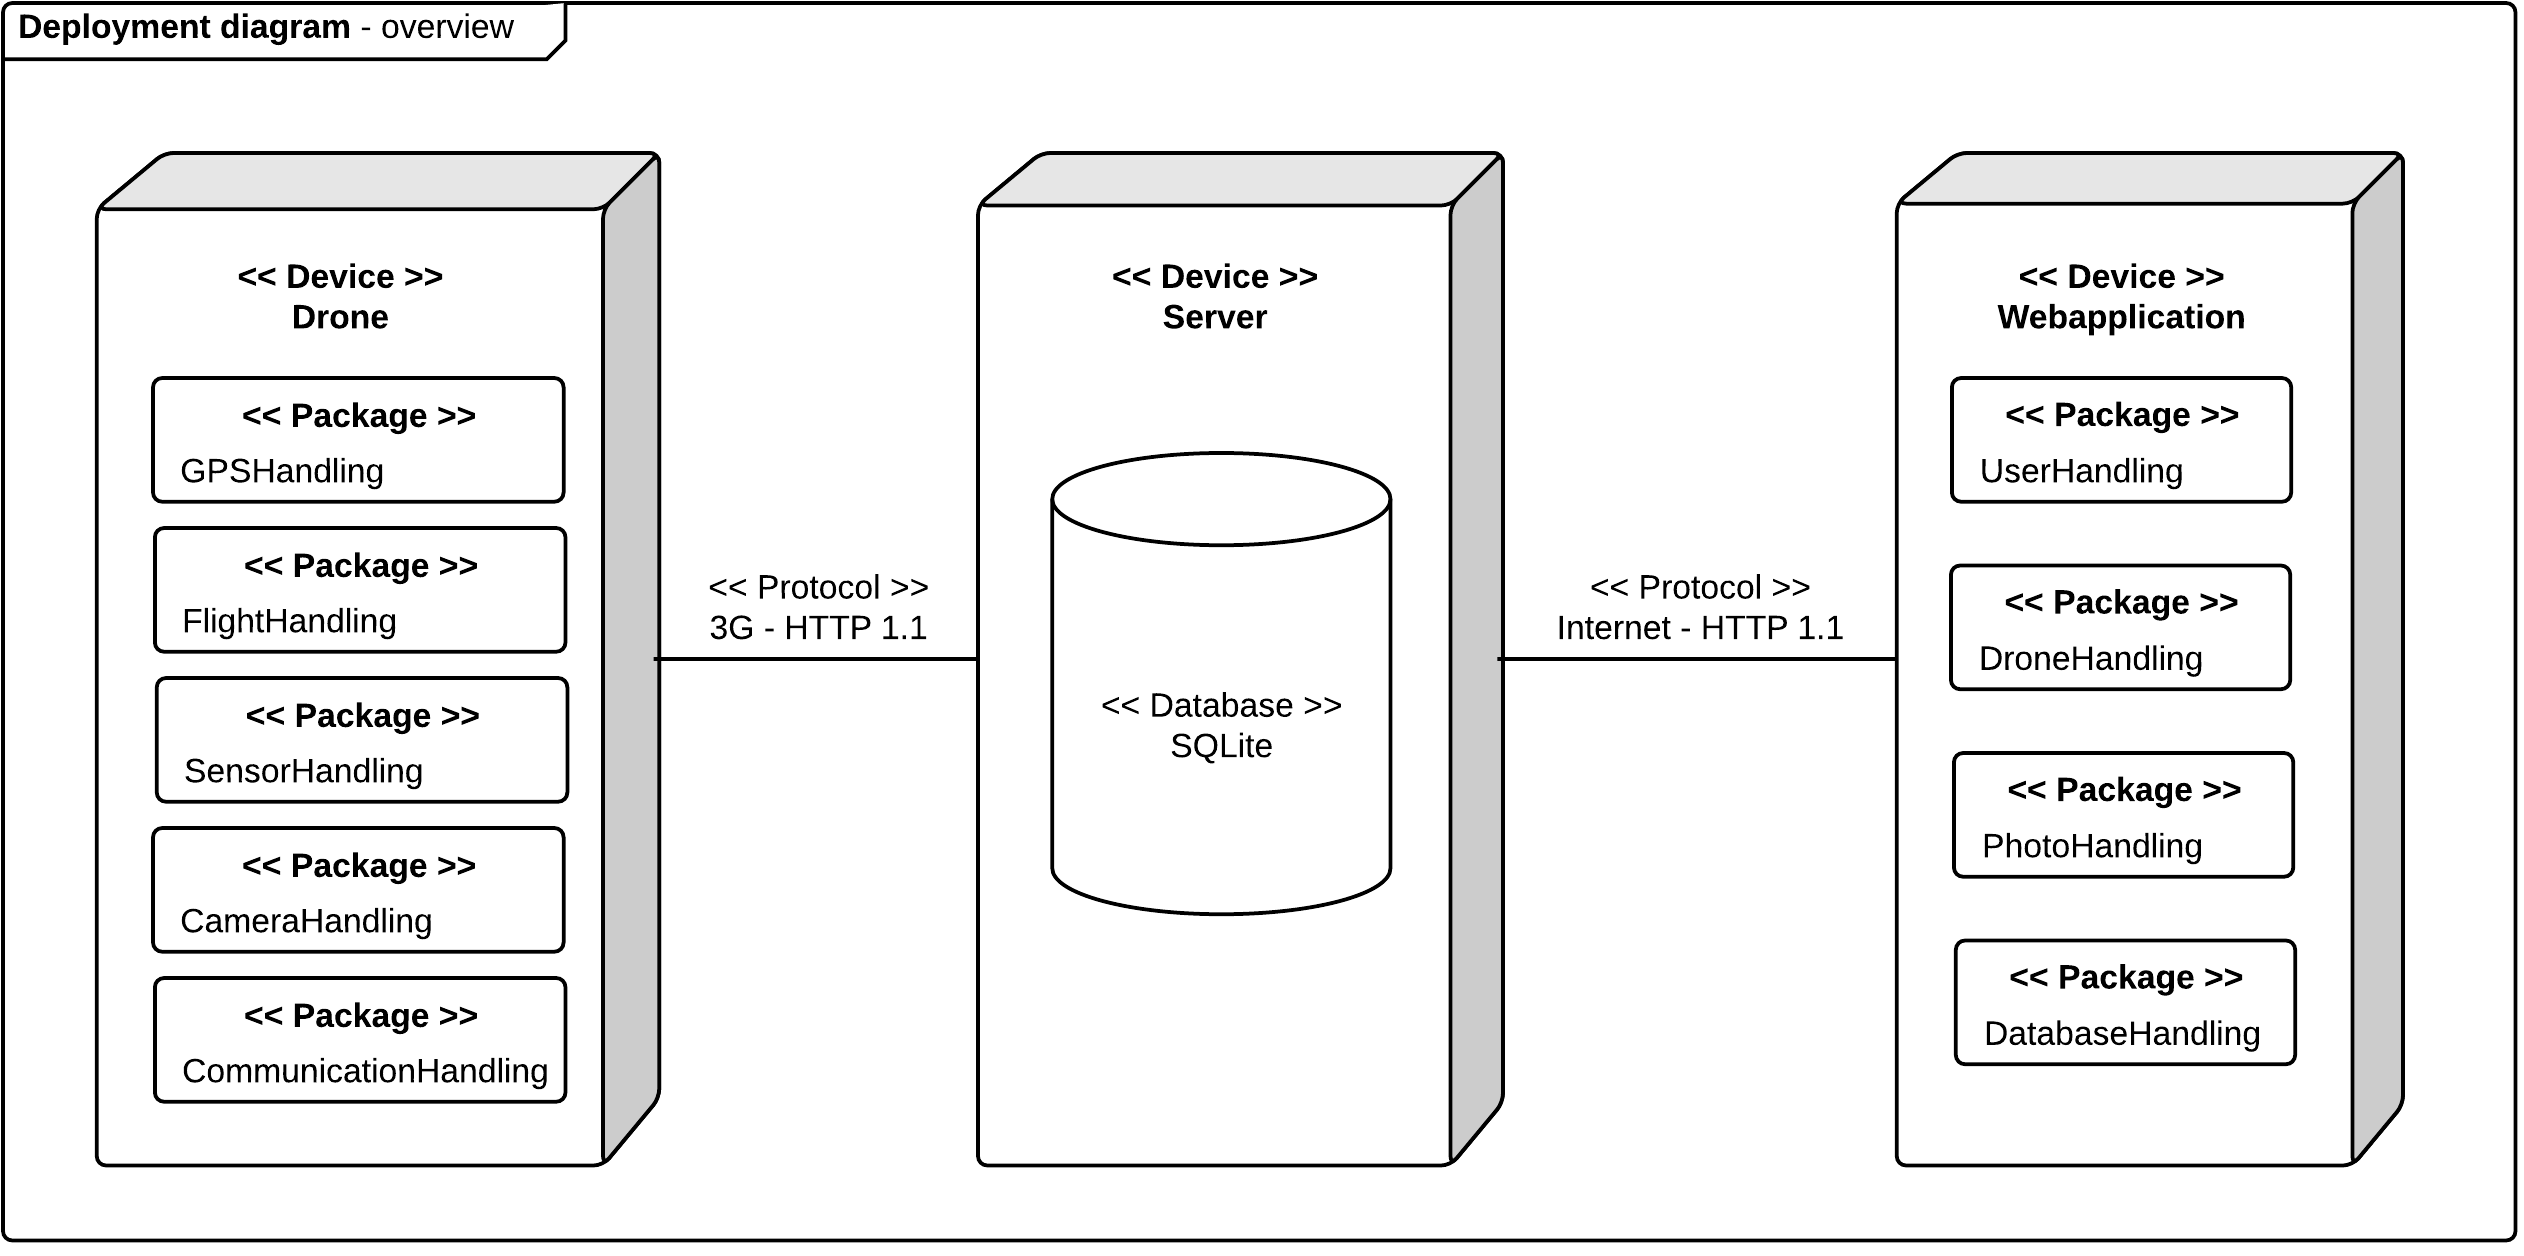
\includegraphics[width=1\textwidth]{Billeder/deployment_overview.png}
\vspace{-0.5cm}
\caption{Deployment diagram}
\label{fig:deployment_diagram}
\end{figure}
 
\newpage


\subsection{Webapplikation}

Webapplikationen fungerer som grænseflade til systemets bruger. Da det ikke ønskes at alle og enhver kan tilgå webapplikationen, skal bruger logge ind før webapplikations funktionalitet kan benyttes. 

Via webapplikationen kan bruger lave nye flyveopsætninger samt monitorere data og information fra tidligere flyvninger. Da det ikke er muligt at rette eller stoppe en aktuel flyvning, skal bruger være opmærksom på hvordan en ny flyveopsætning indstilles. 

Mellem server og webapplikation laves en socket connection. Dette betyder at indholdet af webapplikationen opdateres hver gang der der tilføjes eller ændres i eksisterende data på serverens SQLite database. Yderlige information om webapplikation findes i logical og impelmentation view i \textit{Systemarkitektur og Design} i dokumentationen [xx].


\subsection{HTTP protokol}

Den kommunikationsprotokol der bruges til at sende og modtage data fra server ønskes benyttet af både webapplikation og drone. Da der kun skal laves et interface til server, hvis drone og webapplikation benytter samme protokol.

Webapplikationen kan benytte stort set alle kommunikations protokoller, mens 3G/GPS modulet kun kan benytte et begrænset antal.

Det vælges at benytte HTTP protokollen, da 3G/GPS modulet understøtter denne protokol og fordi protokollen er blandt de mest anvendte protokoller til kommunikation mellem webapplikationer og servere.

Ønskes mere yderlige viden om HTTP protokollen henvises til wikipedia [x] \footnote{http://en.wikipedia.org/wiki/Hypertext\_Transfer\_Protocol} mens der henvis til deployment view i \textit{Systemarkitektur og Design} hvis der ønskes mere viden om brug af protokollen [xx]. 

\newpage
\chapter{Implementation}
Implementering af systemets funktionalitet tager udgangspunkt i de udarbejdede hardware- og softwarediagrammer. Hardwarediagrammer bruges til at definere hvordan systemets hardware kobles, mens softwarediagrammerne bruges til at definere og implementere software.

Implementeringsfasen udarbejdes iterativ, og de højst prioriterede use cases implementeres først. 
Dette afsnit beskriver implementering af systemet.


\section{Drone}
Drone indeholder alt systemets hardware. Software til drone er udviklet i programmerings sproget C++, og er opdelt i forskellige ansvarsområder. Nogle softwareklasser bruges til at aflæse data fra højdesensor, 3G/GPS modul og kompas, mens andre klasser er ansvarlige for kommunikation. Information fra de forskellige softwareklasser samles og behandles på dronens main controller. Ud fra den indsamlede data tilpasses dronens flyveindstilling via dertil indrettede klasser. 


\section{Server}
Indledningsvis i implementeringen blev der lagt meget fokus på server, da den spiller en afgørende rolle i kommunikationen mellen drone og webapplikation. 
Server er udviklet i programmerings sproget Python og med webframeworket Django[x].
Tilsammen udgør Python og Django en SQLite database med et RESTful API. Der benyttes en række API-endpoints for at tilgå eller ændre data på server.

\section{Webapplikation}
Webapplikationen  er udviklet i programmerings sprogene HTML, CSS og JavaScript. Webapplikationens frontend er udviklet med frameworket AngularJS[X], som er et meget vidt benyttet framework udviklet af Google. Derudover benyttes et google maps API til webapplikationen, dette muliggør brugen af kort på webapplikationen. Da AnjularJS er benyttet til udviklingen, er projektet opdelt efter MVC-modellen[x]. 

Kortet er implementeret ved brug af et google-maps directive[X], dette pakker google maps api'et ind og derved gør det mere effektivt i forbindelse med Angular udvikling. Dette betyder også at noget funktionalitet som google maps tilbyder kan ikke direkte bruges i dette directive. Da det var et krav at waypoints skulle oprettes ved klik på kortet, blev der udviklet et specifik klik event på kortet. Når et klik på kortet finder sted bliver der tegnet et waypoint på kortet og i koden bag bliver der oprettet to waypoint objekter. Det ene waypoint objekt er til kortet, dette objekt indeholder kun icon, latitude og longitude til hvor waypointet skal tegnes. Det andet waypoint der bliver oprettet er det waypoint som skal benyttes og sendes til serveren når brugeren ønsker at publicere det tegnede rute. Dette er nødsaget da google-maps directivet ikke kan finde ud af at tegne waypoints hvis de indeholder data som directivet ikke kender til. Figur \ref{fig:click_event} illustrere hvordan klik eventet opretter to waypoint objekter.

\vspace{-5pt}
%kommentar
\begin{figure}[H]
	\centering
	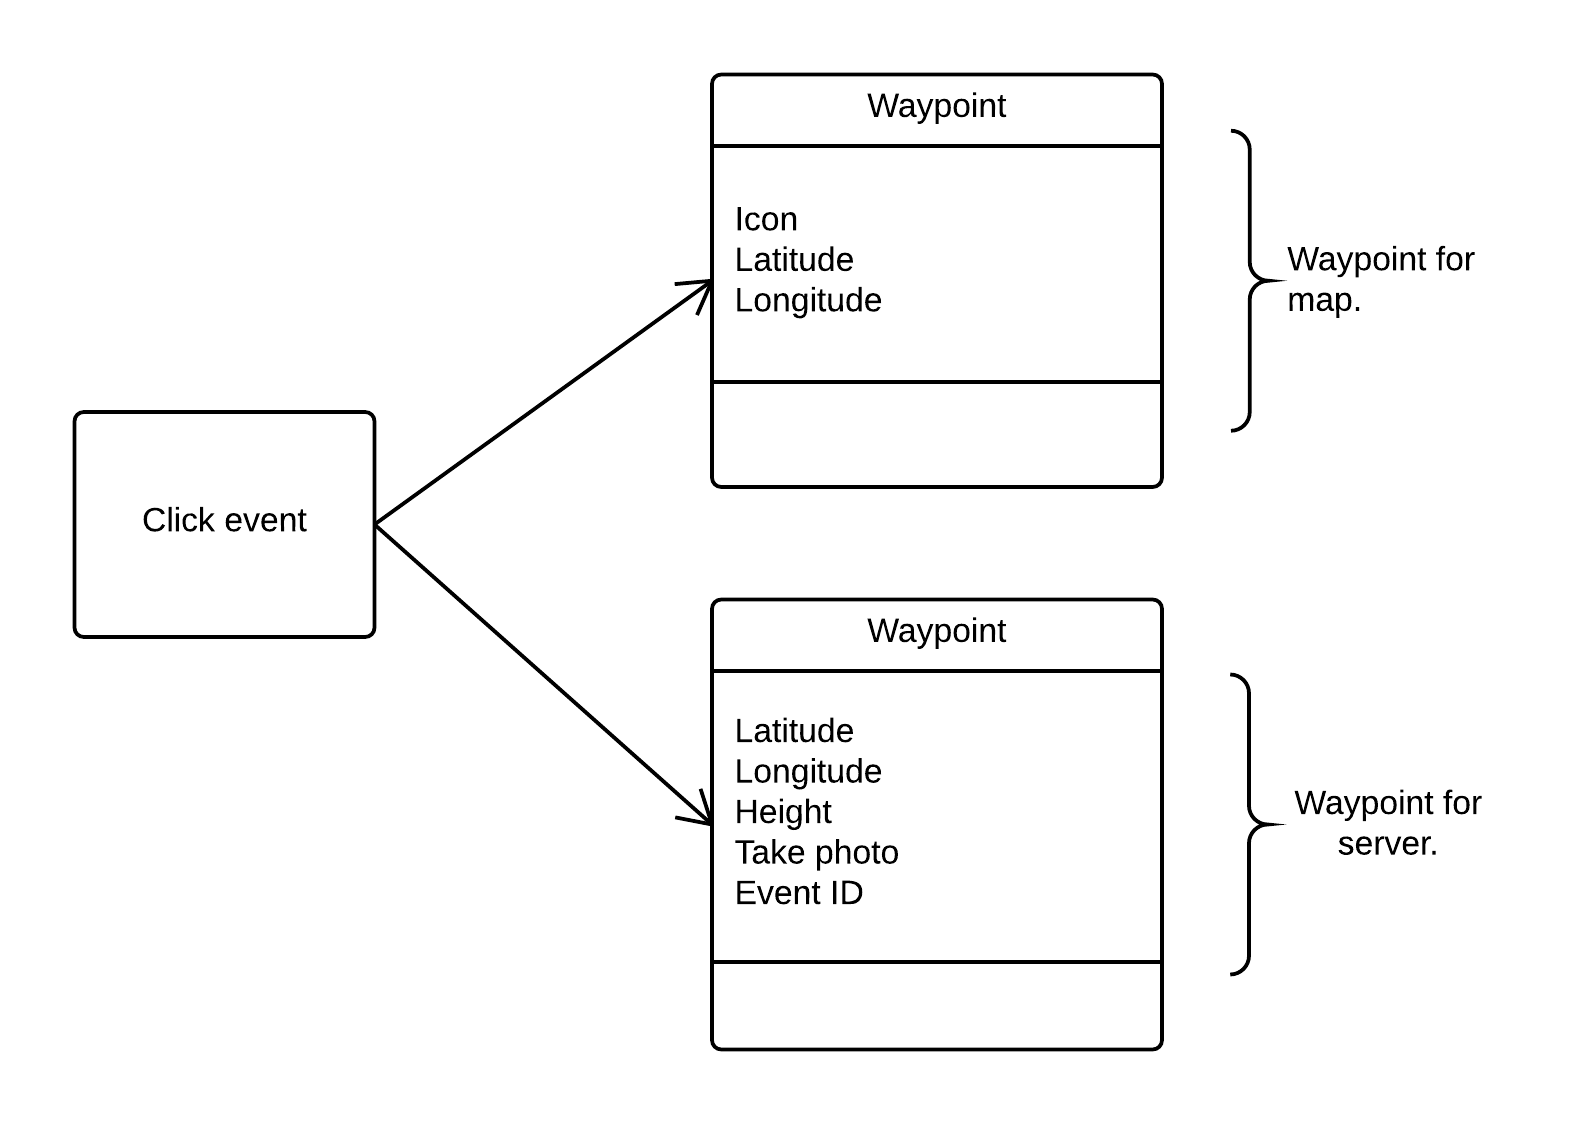
\includegraphics[width=0.6\textwidth]{Billeder/click_event.png}
	\vspace{-5pt}
	\caption{Click event eksempel}
	\label{fig:click_event}
\end{figure}

\newpage
%%%%%% Test %%%%%%
\section{Test}

\label{chap:test}

I projektforløbet er der løbende blevet udført test. Indledningsvis udføres enhedstest i takt med nye moduler/enheder udvikles, senere laves integrationstest der tester kommunikation og samarbejde mellem flere enheder og til sidst udføres accepttest.

Nedenfor ses en kort beskrivelse af de udførte tests:\\


\textbf{Enhedstest} \\
Enhedstest udføres løbende i takt med nye enheder udvikles. Testene udarbejdes for at sikre kvalitet, funktionalitet og grænseflader i de nyudviklede enheder. 

Hovedformålet med enhedstest er at teste tidligt i projektforløbet for at opdage eventuelle fejl og mangler. Hvilket i sidste ende kan spares meget tid og besvær, da fejl og mangler ofte er svære og mere tidskrævende at rette sent i et projektforløb.


\textbf{Integrationstest} \\
I integrationstest testes koblingen mellem to eller flere enheder. Her testet om grænseflader mellem enhederne fungerer og om enhederne kan kommunikere og arbejde sammen.  



\textbf{Accepttest} \\
Accepttesten er en todelt test der tester systemet som helhed. 
Først udføres accepttest af funktionelle krav og dernæst testes ikke-funktionelle krav.
Accepttest af funktionelle krav foregår via en gennemgang af use cases, som bruges til at kontrollere systemets funktionalitet. Ikke-funktionelle krav bruges til at teste systemspecifikationer.  

For yderligere og konkret information om de forskellige tests og tilhørende resultater henvises til testdokumentet[X] i dokumentationen.

\newpage
%\section{Fortræffeligheder}
Dette afsnit har til formål at beskrive hvilke fortræffeligheder der har fundet sted under udviklingen af Autonom overvågningsdrone projektforløbet.

Det er en fortræffelighed at hele systemet er opbygget modulært, systemet er opbygget af tre blokke. En drone, en server og en webapplikation, der er meget lav kobling imellem disse tre enheder i systemet. Med denne lave kobling er det muligt at udskifte dele af systemet udafhængigt at de andre dele. 

Med serveren som en central kommunikations enhed i systemet giver dette også mulighed for at tilføje flere enheder, så som flere droner og/eller flere clienter. Med serveren som kommunikations medie mellem drone og client, bliver alt data også gemt, hvilket muliggøre historik over flyvninger osv. 

Da gruppens medlemmer har forskellige baggrunde, har synagien mellem medlemmerne også fungeret godt og har kunne komplimentere hinanden. 

\newpage
\section{Resultater}

I dette afsnit beskriver resultatet af accepttesten som blev foretaget i projektets afsluttende fase. 
Accepttesten er bygget op om seks test cases, som bruges til at teste det samlede systems funktionalitet. For mere information om de forskellige test cases henvises til test dokumentet. [X] \\

Test case 1 er succesfuldt gennemført. Når dronen tændes, initieres main controller samt 3G/GPS modul og dronen opdaterer sin nuværende GPS position. Efter at have opdateret egen GPS position opretter dronen forbindelse til mobilt 3G-netværk og sender information om sin nuværende GPS position til server.

Test case 2 er delvist gennemført. Bruger har mulighed for at tilgå webapplikation, logge ind på applikationen og oprette nye flyveopsætninger. Webapplikationen kan både hente og vise information fra server. Det er dog ikke muligt at sende information fra webapplikation til server, da kommunikation mellem webapplikation og server ikke er fuldt ud implementeret. Hvilket betyder at bruger ikke kan uploade nyoprettede flyveopsætninger til server.  

Test case 3 er ligesom test case 2 delvist gennemført. Dronen kan sende sin nuværende GPS position til server og hente flyveopsætninger fra server. Det bemærkes dog, at flyveopsætninger, der hentes fra server, ikke er oprettet via webapplikationen men derimod tilføjet server via backend. 
Tilpasning af flyveindstillinger er implementeret i tre trin. Først tilpasses flyvehøjde, dernæst tilpasses flyveretning og når både flyvehøjde og flyveretning er tilpasset flyves fremad.
Tilpasning af flyveindstillinger er ikke blevet optimeret, hvilket får dronen til at afvige fra det ønskede resultat og gør dele af test case 3 fejler.

Test case 4, 5 og 6 er ikke godkendt, da funktionalitet kun er designet og ikke implementeret.


\newpage
\section{Dikussion af resultater}

I dette afsnit beskrives og diskuteres de resultater gruppen opnåede og der laves en beskrivelse af de punkter der kunne være lavet på bedre, smartere eller anderledes vis. Diskussionen tager udgangspunkt i de opnåede resultater beskrevet i resultatafsnittet.

Accepttesten forløb stort set som planlagt indtil test case 4-6 som omhandlede opsamling af billeder, visning af billeder og tilføjelse af antikollision. Test case 4-6 blev ikke godkendt, da de kun blev designet og ikke implementeret. Da arbejdsprocessen var planlagt i iterationer, var de fejlene test cases ikke kritiske for det resterende system.\\

\textbf{Drone}\\
Drone kan under flyvning finde nuværende flyvehøjde, flyveretning og GPS position ved aflæsning af data fra ultralydssensor, kompas og GPS.  Ud fra det aflæste data tilpasses flyveindstillinger. Via det mobile 3G-netværk sender drone information om nuværende position til server og henter flyveopsætninger fra server

Tilpasning af flyveindstilling er implementeret som en tre-trins-raket. Først tilpasses flyvehøjde, dernæst tilpasses flyveretning og når både flyvehøjde og flyveretning er tilpasset flyves fremad. Hver del er implementeret og fungerer hver for sig selv, men samlet set fungerer det ikke optimalt pga. manglende optimering. Til justering og optimering af flyvehøjde og flyveorientering kunne der med fordel være gjort brug af PID regulering.  I implementerings fasen opstod problemer med timing, specielt når 3G/GPS modulet blev brugt. Ved at indføre brug af flertrådet main controller kunne disse problemer undgås. \\

\textbf{Webapplikation}\\
Før systemets bruger kan få lov at tilgå webapplikationens funktionalitet er login påkrævet. Når bruger er logget ind kan der laves flyveopsætninger. Det er lykkes at implementere webapplikationen så den kan hente og fremvise data fra server. 
Men pga. manglede implementering kan webapplikationen ikke sende data til server.\\


\textbf{Server}\\
Server er implementeret med fuldt fungerende database og tilhørende interface. Billeder i databasen er koblet op til events, de kunne med fordel være koblet til waypoints.

